In the previous chapter, we described an I/O deduplication and reduction
mechanism called DRIVE and presented its trace-based evaluation within 
a custom simulator, called \texttt{SimReplay}. The traces we used were
the three (\textit{homes}, \textit{mail}, \textit{webvm}) 21 day-long 
production traces available at \cite{iodedup-online}, from which we 
concluded that the DRIVE system could perform exceptionally well for
the \textit{webvm} trace. However, to further stress the system's
functioning as well as to understand its limits, we need to test it
with more real-world traces. In this chapter, we build the case
for generating synthetic I/O deduplication benchmarks for more
comprehensive evaluation of I/O deduplication techniques.

\section{Motivation}
In general, we can intuitively understand that higher the amount of
duplicate content in the traces, higher the effectiveness of any 
I/O deduplication technique as compared to the Vanilla case. 
However, as our previous evaluation
has shown, even though the \textit{webvm} trace had high levels 
of duplicate content and was an ideal candidate to benefit from
I/O deduplication techniques, the deduplication benefits achievable 
for it was extremely poor
within the IODEDUP system while being exceptionally good within
the DRIVE system. This seems to indicate that it is not just 
the degree of duplicate content but possibly other characteristics
of the \textit{webvm} trace also that contribute to such varied performance.

In our pursuit to test the DRIVE system further, we 
were faced with the following options:-
\begin{itemize}
	\item \textbf{Trace collection toolkit}: Build our own tracing toolkit (\texttt{preadwritedump}) to capture more traces. 
	\item \textbf{Capture production traces}: Deploy above toolkit on production servers to capture real-world traces
	\item \textbf{Capture synthetic benchmarks}: Deploy above toolkit to capture synthetic benchmark traces 
	\item \textbf{Dataset survey}: Perform an exhaustive literature survey to determine if there are any other real-world datasets available that can be used for I/O deduplication performance benchmarking
	\item \textbf{DRIVE evaluation using datasets}: If public datasets or traces available, use them for further testing of DRIVE system
	\item \textbf{Dataset characterization}: Extensively characterize the available traces to learn which particular properties of the \textit{webvm} trace contributed to its enhanced performance in the DRIVE system
	\item \textbf{I/O deduplication benchmarks}: If public datasets are not available, build a case for creating synthetic I/O deduplication benchmarks
\end{itemize}

In the rest of this chapter, we describe the work done 
in pursuing each of these options, and which finally 
builds a case for creating synthetic and realistic
I/O deduplication benchmarks.

\subsection{Building custom trace collection toolkit}
Of the above alternatives, we started off with building our own tracing 
toolkit with a view to deploying it on production servers within our
department. We built the toolkit called \texttt{preadwritedump}, however, 
we were unable to obtain requisite permission from the systems 
administrators to deploy the same on the departmental servers. Although
we could not fully utilize the developed tool, we believe that it would
be helpful for future tracing efforts. Moreover, if we wish to develop
sub-block level deduplication techniques, we need to have a tracing tool
that can perform block-level tracing and dump of I/O content, because 
merely dumping hashes of the blocks is not suitable for sub-block duplicate
identification. With this in mind, we have presented the design and 
implementation of our toolkit in the Appendix~\ref{chap:thesis-tracing}
of this thesis.

\subsection{Tracing of synthetic benchmarks}
The next alternative was to generate 
synthetic workloads and capture corresponding 
traces. However,
the challenge here is to develop synthetic traces that are ``realistic''. 
For example, many public storage and I/O benchmarks exist, however, their 
focus is only on the number of I/Os that can be
generated per second, and not on the actual content being read or written. 
Hence, these benchmarks tend to generate ``realistic'' workload levels (i.e., number of IO 
operations per second) while paying scant attention to
whether the content being generated as part of the read and write 
operations are also realistic or not.
For example, these benchmarks may generate randomized content~\cite{postmark}
or heavily duplicate content~\cite{rubis}
or even write zeros~\cite{zeros}, in some cases. 
For our purposes, usage of benchmarks that write randomized content
will result in very low duplicates in the workload, whereas those that heavily 
generate duplicate content or simply write zeros will overestimate the benefit of deduplication.
Hence we conclude that, existing public benchmarks, though purported 
to be ``realistic'' are not realistic in terms of the content generated
for the I/O and hence are not useful for evaluation of deduplication techniques.

With respect to the use of existing benchmarks for deduplication study, 
it deserves mention that benchmarks like HiBench~\cite{hibench} and RUBiS~\cite{rubis}
have been used in earlier works~\cite{deduping-hibench}
for storage duplicate characterization, wherein 
high levels of duplicate content were reported (eg. 70-80\% duplicate
content observed in RUBiS benchmark). 
However, we take a critical view towards such work because the
intended usage of these benchmark applications (eg. RUBiS~\cite{rubis})
is the study of application performance,
with zero focus on the application's content characterization. 
Basically, these benchmarks generate either heavily-duplicate 
or heavily-random content because the content is irrelevant for the benchmark's intended usage.
However this lack of ``realistic content characterization'' disqualifies their use
for evaluating content deduplication techniques.
Specifically, RUBiS is an application benchmark mimicking
an e-commerce website where most of the content pages are dummy pages, and
hence tend to have repetition of content (eg. repetitive ``item descriptions'' or
``comments'') just to populate the web pages. This content
should not be considered as legitimate duplicate 
content,
%\textemdash{}it is only duplicate
%because content characterization of the application has not been captured in
%the benchmark\textemdash{}
since real e-commerce applications would 
typically not consist of dummy repetitive comments.
Alternatively, the duplicate data created in HiBench benchmark is for 
the express purpose of storage availability in 
bigdata or MapReduce environments, 
hence deduplicating such blocks on storage is counter-productive.  

\subsection{Survey to identify relevant public datasets}
Due to above unsuccessful attempts at generating synthetic workload traces
for evaluation of DRIVE, we once again turned towards datasets in literature
and performed an extensive survey to determine whether any 
relevant useful datasets are available online. 
To begin with, we classified the dataset surveyed into
two sets: (i)~\textit{Public datasets}\textemdash{}these traces are publicly available
online and can be used by any researcher with an Internet connection,
(ii)~\textit{Proprietary datasets}\textemdash{}these are datasets mentioned in various
papers, however they have not been made publicly available. For example, 
the research groups from NetApp, IBM, etc use trace datasets that are 
internally available to them, but are not published online. We describe
the surveyed datasets in Section~\ref{sec:architectingchap-survey}.

After performing the dataset survey with a very wide net, we conclude that 
there are no datasets available for testing I/O deduplication techniques
apart from the ones that were provided at \cite{iodedup-online} which we
have already used. Further, we conclude that the next best way of
preparing datasets for evaluation would be to synthetically generate 
realistic workload traces by capturing the characteristics of the 
available trace itself. 

\subsection{Synthetic generation of realistic traces}
We performed another detailed
literature survey of relevant papers that develop a workload model
based on measurements from real-world, and then 
generate synthetic realistic benchmarks using
the developed model. The survey revealed that there is related work
that generates realistic benchmarks for I/O access (i.e. only concerned
with block numbers accessed, not their content) as well as for storage 
deduplication (i.e. concerned with content stored on disk, not content 
accessed). However, there is no related work so far that generates
realistic I/O access traces that account for the content as well. 
\\
\\
In the rest of this chapter, we build the case for 
\textbf{I/O deduplication benchmarks}
using the conducted survey results, and establish the generation of realistic
benchmarks as useful future work. First, we present the results of our
dataset survey which shows that there are no suitable datasets available
publicly. Next, we present a detailed trace characterization of the 
available \textit{webvm} traces~\cite{iodedup-online} and finally, we make the
case that the detailed trace characterization can be used for generating
realistic benchmarks for evaluation of I/O deduplication techniques.

\section{Survey of datasets and benchmarks in literature}
\label{sec:architectingchap-survey}

\begin{figure*}
	\centering
	\subfloat[Conference-name tag cloud]{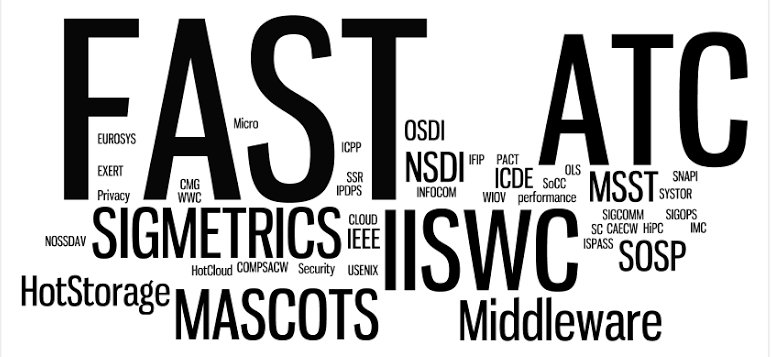
\includegraphics[scale=0.25]{presyn-figures/conference-names-wordle.jpg}} \hfill
	\subfloat[Year-of-publication tag cloud]{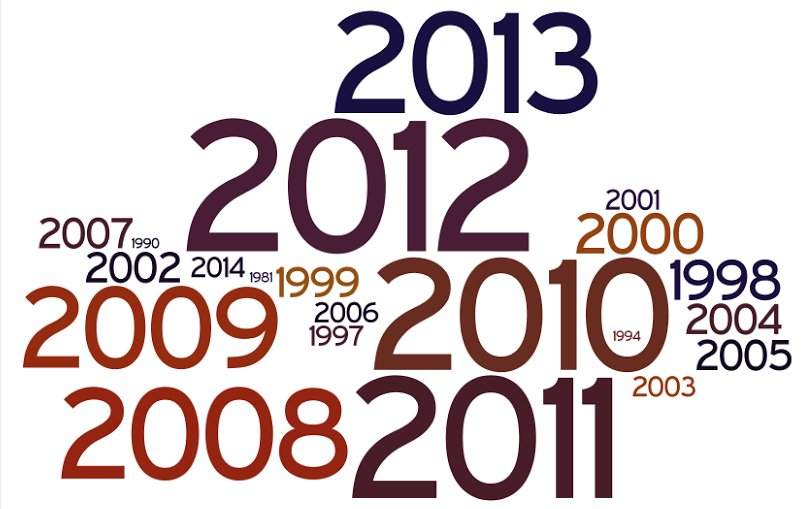
\includegraphics[scale=0.25]{presyn-figures/year-of-publication-wordle.jpg}}
	\\
	\caption{Representation of the conferences and the years of publication covered in our survey}
	\label{fig:tag-clouds}
\end{figure*}


%In the course of the dataset survey, 
We surveyed the datasets used in over
100 publications amounting to a total of over 350 datasets. A similar survey
for storage deduplication datasets (covering 120 datasets from 33 research 
papers) is presented in \cite{generating-datasets}, wherein the requirements
specified for such datasets is that they should be realistic, 
sufficiently large, as well as easily accessible/distributed to 
other researchers. 

The paper \cite{generating-datasets} does not
mention by name which publications were surveyed by the authors, except for 
stating that the 33 research papers were from top conferences from the
years 2010 and 2011. Due to such limited information available, we 
undertook the survey all over again, while at the same time not restricting
ourselves to only a couple of years\textemdash{}instead, we cast a wider net for our
survey by including all papers that were related to any of the following
topics:- (i)~Storage deduplication\index{Storage deduplication}, 
(ii)~Memory deduplication\index{Memory deduplication}, 
(iii)~Storage characterization, and 
(iv)~I/O characterization.


Since the number of papers considered in our survey is huge (more than 100),
instead of listing out the conference names and the year of publication, we
present the following tag clouds (refer Fig.~\ref{fig:tag-clouds}(a) and (b))
which are meant to represent the survey\index{Survey} 
coverage. As can be seen from the
tagcloud in Fig.~\ref{fig:tag-clouds}(a), our survey covers the
important conferences in the areas of storage and workload characterization,
namely \textbf{FAST}, \textbf{ATC}, \textbf{SIGMETRICS} and \textbf{IISWC},
to name a few. Moreover, the years of publication (refer 
Fig.~\ref{fig:tag-clouds}(b)) for the surveyed papers
are mostly within 2009 to 2014, with a few lying even beyond as well.
With this wide coverage of conferences and years of publication, we are
positive that we have covered the necessary ground for this survey.

As mentioned earlier, we classify
the dataset surveyed into two sets (i)~\textit{Public datasets} and
(ii)~\textit{Proprietary datasets}, and for each of these sets, we 
need to distinguish the dataset further based on whether they are one of 
the following:
\begin{enumerate}
	\item I/O traces with content representation, 
	\item I/O traces without content representation,
	\item Storage metadata\index{Metadata} with content representation, or
	\item Storage metadata without content representation
\end{enumerate}
The first item in the above list is the kind of trace we are looking for,
i.e. I/O activity traces with content representation. However, we found
that almost all of the public datasets available online fall in one of 
the other three categories listed above.

\subsection{Public dataset repositories}\index{Dataset repositories}
By the term \textit{public datasets}, we allude to those datasets or 
traces that have 
been made available online by the respective owners. 
A popular repository for
storage and I/O traces is the SNIA-IOTTA Repository~\cite{snia-iotta-repo} which 
is a collection of traces from multiple publications maintained under
the Storage Network Industry Association's Input/Output Traces, Tools and 
Analysis Technical Work Group. Another popular repository
is the one maintained by HP Labs~\cite{hplabs-repo} which 
contains many tools and benchmarks as well, in addition to traces. 
Note that, there are several other small repositories, each hosting the traces 
or datasets for a single or few publications, we list them separately in 
the next section under \textit{Public individual datasets}.
Below we provide a listing of those online trace repositories, 
which contain huge number of traces (i.e. multiple trace sets, not just one)
and are available to the researchers for development and analysis of network 
and storage systems.
\begin{enumerate}
	\item \textbf{SNIA IOTTA Repository}~\cite{snia-iotta-repo}: collaborative effort under SNIA IOTTA TWG to provide storage-related I/O traces, tools and analysis to the entire research community free of cost.
	\item \textbf{HP Labs Repository}~\cite{hplabs-repo}: provides several file system and application traces captured using HP Labs' tools like DataSeries and Lintel. However, some of these traces are very old, and may not be representative of current systems.
	\item \textbf{UMass Trace Repository}~\cite{umass-repo}: provides network, storage, and other traces, some of which are generated at UMass while some others are donated.
	\item \textbf{Internet Traffic Archive}~\cite{ita-repo}: provides access to traces of Internet network traffic. 
	\item \textbf{VMware image repository}~\cite{thoughtpolice-repo}: provides many VMware images with various Linux distributions installed like CentOS, Debian, Fedora, FreeBSD and OpenSUSE.
	%\item FSL labs repository
	%\item LiveDFS repo?
\end{enumerate}

Next, we discuss the suitability of the traces, hosted at 
each of the above public dataset repositories, 
for the purpose of I/O deduplication evaluation.

\subsubsection{1. SNIA IOTTA Repository traces}
This repository contains several trace sets including Block I/O traces, NFS 
traces and System call traces. The publications that make use of these 
traces are~\cite{flexi-replay, iodedup, animation-nfs, winservers, metadata-evolution, tracefs}, among which \cite{iodedup} is the only paper which deals
with I/O deduplication-related traces\textemdash{}none of the other trace sets at
this repository have data content representation, and hence they are not
suitable for evaluating I/O deduplication techniques.

\subsubsection{2. HP Labs Repository traces}
This repository contains several file system and application traces, however
some of these traces are very old, and also none of these traces have any
content representation either.

\subsubsection{3. UMass Trace Repository traces}
This repository provides traces for network, storage, memory, etc and is a 
collection of traces used in various publications like~\cite{flexi-replay, 
intradisk-parallelism, memorybuddies}. Apart from the traces provided 
of memory contents, none of the other traces in this repository has any
content representation. Moreover, the memory traces are also published 
as snapshots of memory contents and not in the form of an I/O trace, 
indicative of which block is being inserted or evicted from cache at 
which time. Hence, even these traces are not suitable for evaluation of
I/O deduplication techniques.

\subsubsection{4. Internet Traffic Archive traces}
This repository provides access to traces of Internet network traffic, for
potential characterization, benchmark generation, etc and even though
a few of these traces (eg. LBL-TCP-3, LBL-PKT) are packet traces, instead
of just web requests or HTTP traces, however they still do not represent
the packet content or payload. Hence, none of these traces are suitable
for I/O deduplication analysis, not even as synthetic workloads.

\subsubsection{5. VMware image repository}
This is a repository of 78 VMware virtual machine images with various
Linux distributions installed in the default configuration. This 
repository has been used in a few publications~\cite{p-dedupe, ddelta} to
motivate storage deduplication and compression. However, since these
are static images and not I/O workloads in themselves, they are not
suitable for evaluation of I/O deduplication techniques.

\subsection{Public individual datasets}
These are individual datasets that were used for the 
characterization and evaluation in a couple of papers
and have been made available online for use by other researchers.
\begin{enumerate}
	\item \textbf{I/O deduplication traces}~\cite{iodedup-online}: Traces provided by the I/O deduplication paper~\cite{iodedup} which we also used in our evaluation
	\item \textbf{Plan 9 traces}~\cite{p9-traces}: File system snapshots of the Plan 9 file system deployed in the Computing Sciences Research center of Bell Labs. Has content representation, but is suitable only for storage deduplication studies, not for I/O deduplication
	\item \textbf{Animation-bear dataset}~\cite{animation-bear}: Traces released by HP Labs, collected at a feature animation company\textemdash{}these are NFS traces and have no content representation
	\item \textbf{Linux kernel \& GCC sources}~\cite{kernel-src, gcc-src}: A few papers~\cite{p-dedupe, ddelta} use kernel and GCC sources to perform study of storage deduplication systems, by exploiting the fact that multiple successive versions of the same software tend to have a lot of overlapping content.
\end{enumerate}

Among these, the first dataset (i.e. the I/O deduplication traces at~\cite{iodedup-online})
is the one we have used for DRIVE evaluation in the previous chapter. These
traces are also present at the SNIA IOTTA repository mentioned above, and 
is the only set of I/O access traces which have content representation included.
The remaining traces are all either storage metadata traces or I/O traces
without content representation, hence unfit for evaluation of I/O deduplication
techniques.

\begin{table} [t]
	\begin{tabular}{|l|l|c|c|c|l|} \hline
	\textbf{No.} & \textbf{Dataset} & \textbf{Cited} & \textbf{Related to} & \textbf{Comments regarding} \\
	\textbf{} & \textbf{source} & \textbf{by} & \textbf{I/O, storage} & \textbf{suitability for} \\
	\textbf{} & \textbf{} & \textbf{} & \textbf{or memory} & \textbf{I/O dedup evaluation} \\ \hline
	1 & IODEDUP traces & \cite{iodedup} & I/O & Suitable for I/O dedup evaluation \\ 
	2 & SNIA IOTTA Repo & \cite{flexi-replay, winservers, metadata-evolution, tracefs} & I/O & No content representation \\ 
	3 & HP Labs Repo & \cite{storage-system-security, hplabs-repo} & Storage, I/O & No content representation \\
	4 & UMass Trace Repo & \cite{flexi-replay, intradisk-parallelism, memorybuddies} & Storage, I/O & No content representation \\
	5 & Internet Traffic Archive & \cite{failure-of-poisson, search-for-invariants, ita-repo} & Internet & No content representation \\
	6 & VMware Image Repo & \cite{p-dedupe, ddelta} & Storage & Storage metadata, not I/O \\
	7 & Plan 9 traces & \cite{venti} & Storage & Storage metadata, not I/O \\
	8 & Animation-bear dataset & \cite{animation-bear} & I/O & No content representation \\ 
	9 & Kernel \& GCC source & \cite{p-dedupe, ddelta} & Storage & Storage metadata, not I/O \\ \hline
	\end{tabular}
	\caption{Summary of \textit{public} datasets uncovered in the survey}
	\label{tab:public-listed}
\end{table}

\subsection{Proprietary datasets}\index{Proprietary datasets}
So far we have seen the publicly-available storage and I/O datasets. However,
this is a small fraction of all the datasets that have been used and cited
in all the papers that we surveyed. In other words, most of the datasets that
are used for evaluation in literature are rarely hosted 
publicly~\cite{generating-datasets} or made
available to other researchers for further perusal and analysis. In what
follows, we present a brief categorization of such datasets and cite the
works which have used each dataset category.

\begin{enumerate}
 \item \textit{Homes:} This basically consists of the home directories of 
 several employees or students or researchers hosted on a common or 
 shared storage. The access workload is such that the files are read
 and written by a single user each, although the user may end up 
 making several copies of the same file for purposes of editing, 
 translations, conversions, versioning, etc. Such datasets are used
 in~\cite{primary-data-dedup, backup-workloads-characterization, 
 datadomain, cifs-study, redundancy-alternatives}.
 \item \textit{WebServer:} Consists of traces (storage or I/O) from
 webserver workloads, and includes Web ``search'' workloads also in some
 cases. Such workloads are traced and characterized in several research 
 efforts like~\cite{storagecharacterization, filesystem-workloads, 
 content-sampling, my-cache-or-yours, filesize-distrib-cause, 
 web-cable-modem, scaling-phenomena, web-client-access-patterns}.
 \item \textit{CollaborationShares:} This consists of shared storage
 among a group of researchers or collaborators such that the files
 are created by one user and accessed by many others for read and/or
 updates. This dataset may also have duplicates due to multiple 
 copies for editing and versioning~\cite{content-sampling, idedup, 
 cifs-study, redundancy-alternatives}
 \item \textit{SoftwareDeployment:} This consists of the data from 
 a server which contains VM images, softwares and binaries to be 
 used for deployment by users, and the workload is such that the
 files are created by one or more system administrators and used
 or accessed by a bigger user population. This dataset may have duplicates due
 to similarities across the softwares and/or VM images~\cite{similarity}.
 Such datasets are used for the evaluation of storage deduplication
 in \cite{idedup, redundancy-alternatives}.
 \item \textit{VM-Dataset:} A set of a few hundred VM images with
 installations of different versions of operating systems, applications
 and libraries is considered under this dataset. The similarities
 across VM images are due to multiple VM images being instantiated
 from a single golden master or template image~\cite{similarity, dedup-effectiveness, 
 primary-data-dedup, vdn, building-highperf-dedup}.
 \item \textit{VM-Backup:} This consists of a setup where one or more VMs
 are fully or partially backed up regularly, such
 that the backups would have lot of redundancies amongst them~\cite{ddelta, 
 vmdk-backups, hysteresis-rechunking, lowcost-dedup-for-backup}.
 \item \textit{DatabaseBackup:} Similar to the VM-Backup dataset mentioned above,
 several works also use database backup workloads for evaluation
 of storage deduplication techniques~\cite{ddelta, backup-workloads-characterization, 
	 hybrid-dedup, ventana}. 
\end{enumerate}

\begin{table} [t]
	\begin{tabular}{|l|l|c|l|} \hline
		\textbf{No.} & \textbf{Dataset category} & \textbf{Dataset description} & \textbf{Cited by} \\ \hline
1 & \textit{Homes} & Home directories on shared storage & \cite{primary-data-dedup, backup-workloads-characterization, datadomain, cifs-study, redundancy-alternatives} \\ 
2 & \textit{WebServer} & Traces from webserver workloads & \cite{filesystem-workloads, content-sampling, web-cable-modem, scaling-phenomena, web-client-access-patterns} \\
3 & \textit{CollaborationShares} & Files created by one, read by many & \cite{idedup, cifs-study, redundancy-alternatives, content-sampling} \\
4 & \textit{SoftwareDeployment} & Files created by one, used by many & \cite{idedup, primary-data-dedup, redundancy-alternatives} \\
5 & \textit{VM-Dataset} & Few hundred VM images & \cite{similarity, vdn, primary-data-dedup, dedup-effectiveness, building-highperf-dedup} \\
6 & \textit{VM-Backup} & Full or partial backup of VMs& \cite{ddelta, vmdk-backups, hysteresis-rechunking, lowcost-dedup-for-backup} \\
7 & \textit{DatabaseBackup} & Backup of production databases & \cite{ddelta, backup-workloads-characterization, hybrid-dedup, ventana} \\ \hline
	\end{tabular}
	\caption{Summary of \textit{proprietary} datasets uncovered in the survey}
	\label{tab:proprietary-listed}
\end{table}

We summarize the results of our above dataset survey in 
Table~\ref{tab:public-listed} for \textit{publicly-available} datasets
and in Table~\ref{tab:proprietary-listed} for \textit{proprietary} datasets. 
For each dataset, we identify 
it by a name, and list a few representative reference
papers in which the dataset has been utilized. For each dataset,
we also mention whether it is related to I/O, storage
or memory traces and present comments regarding the dataset's
suitability for use in evaluation of I/O deduplication techniques.

\subsection{Benchmarks}
Some benchmarking\index{Benchmarking} 
tools and application benchmarks have also been used for
workload generation\index{Workload generation} in literature. 
Some of the most popular benchmarks
for Storage I/O workload generation are as under:-
\begin{enumerate}
	\item \textbf{Filebench}~\cite{filebench}: It is a file 
		system and storage 
	      benchmark that can generate both micro and macro workloads. 
	      It allows detailed workload specification using Workload
	      Model Language (WML) as well. It includes several popular
	      macro-workloads like web server, mail server and database 
	      server.
	\item \textbf{dbench}~\cite{dbench}: This tool can be used to stress test
	      a storage system to figure out its saturation performance
	      level. It allows complex load specification, however the
	      point is not to just generate specific load levels, rather
	      the point is to push the storage system to its limits for
	      the purpose of benchmarking its performance.
	\item \textbf{HiBench}~\cite{hibench}: This is a benchmark suite
	      for Hadoop mapreduce application benchmarking,
	      comprising of both micro-benchmarks as well as application
	      workloads like web search, machine learning and analytic
	      querying.
	\item \textbf{IOzone}~\cite{iozone}: This is a file system benchmark
	      tool that generates and measures the performance of a wide
	      variety of file system operations like \texttt{read}, \texttt{write},
	      \texttt{re-read}, \texttt{re-write}, \texttt{random read},
	      \texttt{mmap} and so on.
	\item \textbf{IOMeter}~\cite{iometer}: This is a load generation and
	      characterization tool for both storage and network, and can
	      generate loads on single or multiple systems.
	\item \textbf{PostMark}~\cite{postmark}: This is a benchmark to 
	      emulate and measure the functionality of email servers, 
		  web servers and news servers.
	\item \textbf{FIO}~\cite{fio}: Flexible IO tester (FIO) is a tool that 
		  allows the user to write a job file according to the load that 
		  needs to be simulated, and the tool spawns multiple processes
		  to generate the requested load.
	\item \textbf{CloudSuite}~\cite{cloudsuite}: CloudSuite is a benchmark
		  suite currently consisting of 8 application benchmarks that are
		  based on real-world setups in today's datacenters. The benchmarks
		  supported include data serving, data caching, web serving 
		  benchmarks and so on.
	\item \textbf{TPC Benchmarks}~\cite{tpc}: The Transaction Processing
		Performance Council (TPC) defines benchmarks related to transaction
		processing and databases, which can be used to benchmark the 
		performance of various applications, like OLTP, decision support
		and many more.
	\item \textbf{SPEC Benchmarks}~\cite{spec}: The Standard Performance 
		Evaluation Corporation (SPEC) establishes, maintains and endorses
		a standardized set of benchmarks for high-performance computers,
		like compute-intensive benchmarks, mail server benchmarks (now retired),
		virtualization performance benchmarks, etc.
	\item \textbf{NAS Parallel Benchmarks}~\cite{nasa}: This is a suite of
		programs designed to evaluate parallel supercomputers, at the
		NASA Advanced Supercomputing Division.
	\item \textbf{HPC Challenge Benchmark}~\cite{hpcc}: This is a benchmark
		suite comprising of 7 tests, measuring various metrics like rate of memory
		operations sustainable, total communication capacity of the network,
		latency and bandwidth of simultaneous communications, etc.
	\item \textbf{PARSEC}~\cite{parsec}: The Princeton Application Repository for 
		Shared-Memory Computers (PARSEC) is a benchmark suite containing many
		multi-threaded programs simulating diverse workloads, like image
		processing, financial analytics, and video encoding.
	\item \textbf{Kernel}~\cite{kernel-src} \textbf{and other sources}~\cite{am-utils, emacs} \textbf{compile benchmark}
\end{enumerate}		

Most of the above benchmarks are either too simplistic or have so many 
control knobs that it is a daunting task to choose the correct 
settings~\cite{generating-datasets}. For example, the work in 
\cite{storage-benchmark-coverage} shows that to exhaustively try all
settings in the benchmarks like FIO, IOzone and Postmark is too time
consuming\textemdash{}instead, 
it recommends that only the minimum and maximum
value for every setting need be tested. It makes an arguable assumption 
that the intermediate settings will result in output that lies between
the outputs for the minimum and maximum settings.

Given any benchmarking tool which has several knobs that can be tweaked,
we might still try tweaking the knobs exhaustively to determine those
settings which produce a compatible workload for 
I/O deduplication evaluation.
However, the onus of proving that the resulting tweaked workload is a 
realistic workload\index{Realistic workload} would still loom large. 
Particularly, most of these benchmarks
do not have realistic content representation~\cite{dedis}, 
and generate either highly duplicate (eg. Bonnie++~\cite{bonnie}) 
or highly random content (eg. 
PostMark~\cite{postmark}, Fstress~\cite{fstress}).
We thus make the claim that,
after having established the initial worth of the DRIVE system using
the available traces, there is nothing more to be gained by evaluation
using synthetic benchmarks\index{Synthetic benchmarks}. 
Further evaluation of the DRIVE system is
valuable only if performed using real-world workloads 
or using ``realistic'' benchmarks.

A study of various benchmarks and analysis by ``benchmarking'' of the
benchmarks is done in~\cite{rocket-science}, which shows that most of
the literature consists of researchers using their own customized
or \textit{ad-hoc}
synthetic benchmarks, which results in incomparable results across
papers. This is an undesirable situation, 
and the work in \cite{rocket-science}
proposes that there should first be a consensus regarding the
dimensions to be benchmarked, and then agreement on the methodology
to benchmark each dimension and comparison of results across systems.
It proposes several dimensions for file system benchmarking, like 
\textit{I/O, on-disk, metadata, caching} and \textit{scaling}.
Due to lack of consensus regarding dimensions, and
the unsuitability of most existing benchmarks for IO deduplication
evaluation, we turn to characterizing the available traces instead.


%\begin{figure*}
%	\centering
%	\includegraphics[scale=0.25]{presyn-figures/datasets-classified.pdf}
%	\caption{Classification of publicly-available datasets: \textit{Only one 
%	set of traces falls in the category we are interested in, which is I/O 
%	traces with content representation}}
%	\label{fig:datasets-classified}
%\end{figure*}


\subsection{Summary of survey findings}
The purpose of this survey is to find publicly-available datasets
of I/O traces with content representation. Our survey revealed that
among the publicly-available datasets, only the ones available 
via IODEDUP paper~\cite{iodedup} have content representation,
and we have already used them for our evaluation in the previous
chapter. All other publicly-available datasets lie in one of
the other three categories.
%, as depicted in Fig.~\ref{fig:datasets-classified}.

Based on our findings that (i) existing public datasets are not
relevant for evaluation of I/O deduplication, (ii) many relevant
datasets are proprietary and not publicly-available, as well as,
(iii) existing benchmarks are not ``realistic'' enough for our purposes, 
we turn to the next avenue of using real-world traces to build
synthetic traces ourselves. We performed a detailed literature
survey of this area (i.e., generating realistic traces) and
find that all such efforts rely on trace characterization of some 
available real-world traces, to generate realistic synthetic traces. 
Therefore, next we perform trace characterization of the 
available \textit{homes} and \textit{webvm} traces,
which may be helpful to build realistic synthetic traces in future.


\section{Trace characterization of available dataset} %\cite{iodedup-online}}
\label{sec:architectingchap-tracechar}
In Section~\ref{sec:similarity-study}, we presented a brief study
of content similarity in the IODEDUP traces available online 
at \cite{iodedup-online}, by presenting 
metrics like ``sharing'' factor and content ``occurrence'' factor
for the traces. In this section, we perform a thorough study
to capture more characteristics of the workload
which can be used for synthetic generation of realistic
benchmarks, in future.

We characterize the \textit{webvm} and \textit{homes} traces from \cite{iodedup-online}
using the following four major
metrics for both read and write requests separately. Note that, I/O
deduplication techniques attempt to optimize only the disk read performance,
so it would be preferable to capture the disk read and write characteristics
of the trace separately, rather than together. 
\begin{enumerate}
		\singlespacing
	\item Blocks accessed distribution
	\item Run length distribution
	\item Reuse distribution
	\item Jump length distribution
\end{enumerate}

For each of the above metrics, we first present a basic definition 
accompanied by an example and then present the characterization of the
traces based on that metric. Along-with the block-based interpretation of
the metric, we also present the ``content-based interpretation'', the point
being that I/O deduplication is to be performed for traces that have
duplicate content so the content-defined trace characterization is especially
relevant.

 \begin{table}[t]
 \caption{Summary statistics of one week I/O workload traces \textit{webvm} and \textit{homes}~\cite{iodedup}}
%  \hspace{-0.2in}
 \begin{center}
 \begin{tabular}{|c|c|c|c|c|} \hline
   \bf{Workload} & \bf{Filesystem} & \bf{Memory} & \bf{Filesystem} & \bf{Filesystem size} \\
  \bf{type} & \bf{size (GB)} & \bf{size (GB)} & \bf{accessed (\%)} & \bf{(no. of 4KB blocks)} \\ \hline
  \textit{webvm} & 70 & 2 & 2.8 & 18 million \\
  \textit{homes} & 470 & 8 & 1.44 & 123 million \\ \hline
 \end{tabular}
 \label{tab:tracechar-summary-stats}
 \end{center}
 \end{table}
 

Before presenting the distributions, we present summary
statistics regarding the traces considered in 
Table~\ref{tab:tracechar-summary-stats}\textemdash{}these are statistics reproduced
from the original paper~\cite{iodedup}.
As can be seen in the table, \textit{webvm} trace is from a filesystem of size only 70 GB
whereas \textit{homes} trace has a filesystem of size 470 GB backing it. This implies
that the range of block addresses accessed in the latter filesystem is expected
to be greater than the former. The primary memory allocated in both systems
is also different\textemdash{}2 GB and 8 GB, respectively. Thus, the \textit{homes} trace
has been captured downstream of a much bigger cache than the \textit{webvm}
trace\textemdash{}this may be partly the reason why the \textit{homes} trace does not
seem to have much duplicate content to be exploited by the I/O deduplication
techniques (refer Fig.~\ref{fig:similarity-distrib} in Section~\ref{sec:similarity-study}).

In Table~\ref{tab:tracechar-summary-stats}, the percentage (\%) of 
filesystem accessed indicates that in both concerned systems, 
the total number of block addresses accessed in the trace constitutes only
a small fraction of the entire file system size. This implies that if the
metadata is constructed dynamically (i.e., while the application is 
executing), it needs to represent only that portion
of the filesystem that is accessed in the workload, and not the whole filesystem.
Note that, this requirement is different from that of a storage deduplication
system which needs to persistently retain metadata regarding the entire data
within the system.


 
For trace characterization, we consider the entire three-week \textit{webvm}
and \textit{homes} trace, and report various distributions (instead
of averages) in accordance with the insight in 
\cite{commercial-characterization} that ``distribution matters, not 
the average''. 

\subsection{Blocks accessed distribution}

%These figures were plotted directly from Octave, and hence having all
%this problem. The only thing good in Octave was that it could easily
%plot histogram with 25 bucket by hist(X, 25). Plotting has been a real
%pain though, so better to use [y, x] = hist(X,25) and then print out
%the x and y values, to use them separately in a gnuplot script with
%desired formatting.
%\hspace{-1in}
\begin{figure}[t]
	\centering
	\subfloat[Access distribution of blocks read (\textit{webvm})]{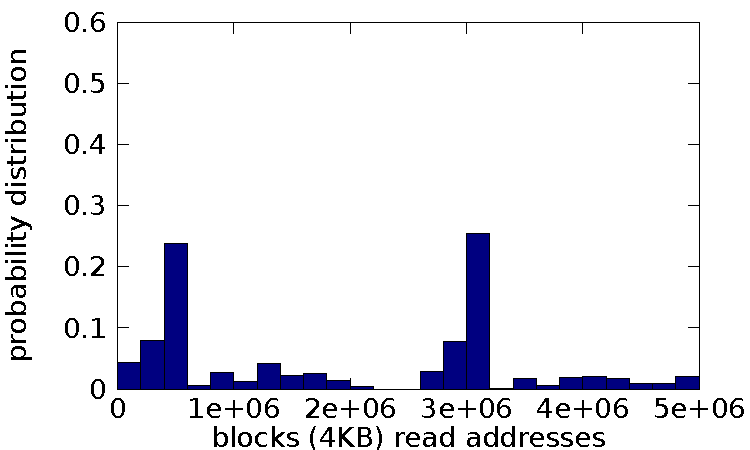
\includegraphics[scale=0.6]{tracechar-figures/21-day/webvm-block-read-appended-21-prob.pdf}}
	\hfill
	\subfloat[Access distribution of blocks written (\textit{webvm})]{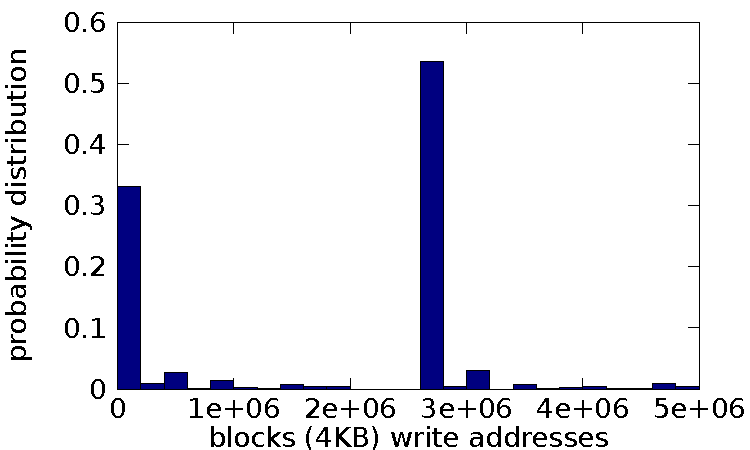
\includegraphics[scale=0.6]{tracechar-figures/21-day/webvm-block-write-appended-21-prob.pdf}}
	\\
	\subfloat[Access distribution of blocks read (\textit{homes})]{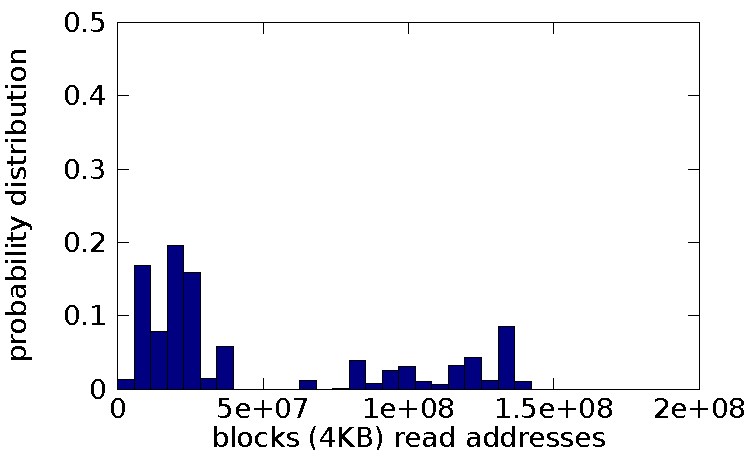
\includegraphics[scale=0.6]{tracechar-figures/21-day/homes-block-read-appended-21-prob.pdf}}
	\hfill
	\subfloat[Access distribution of blocks written (\textit{homes})]{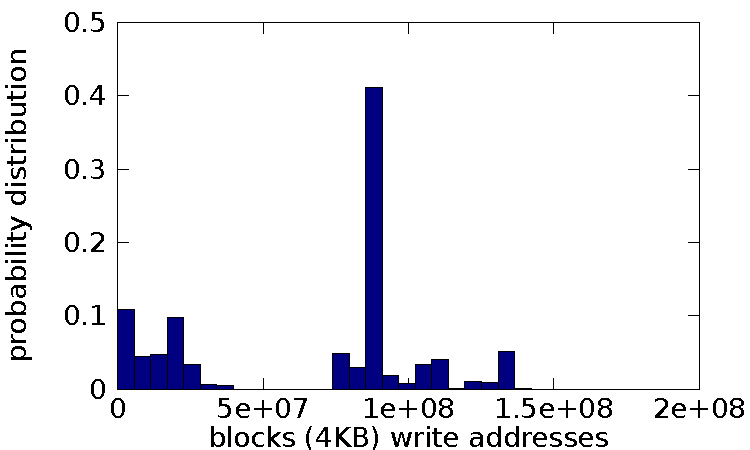
\includegraphics[scale=0.6]{tracechar-figures/21-day/homes-block-write-appended-21-prob.pdf}}
	\caption{Block access popularity distribution for reads and writes in 
	\textit{webvm} and \textit{homes} traces}
	\label{fig:webvm-blocks-read-write-distrib}
\end{figure}

%\hspace{-0.7in}
%\begin{minipage}[t]{0.6\textwidth}
%\begin{figure}
%	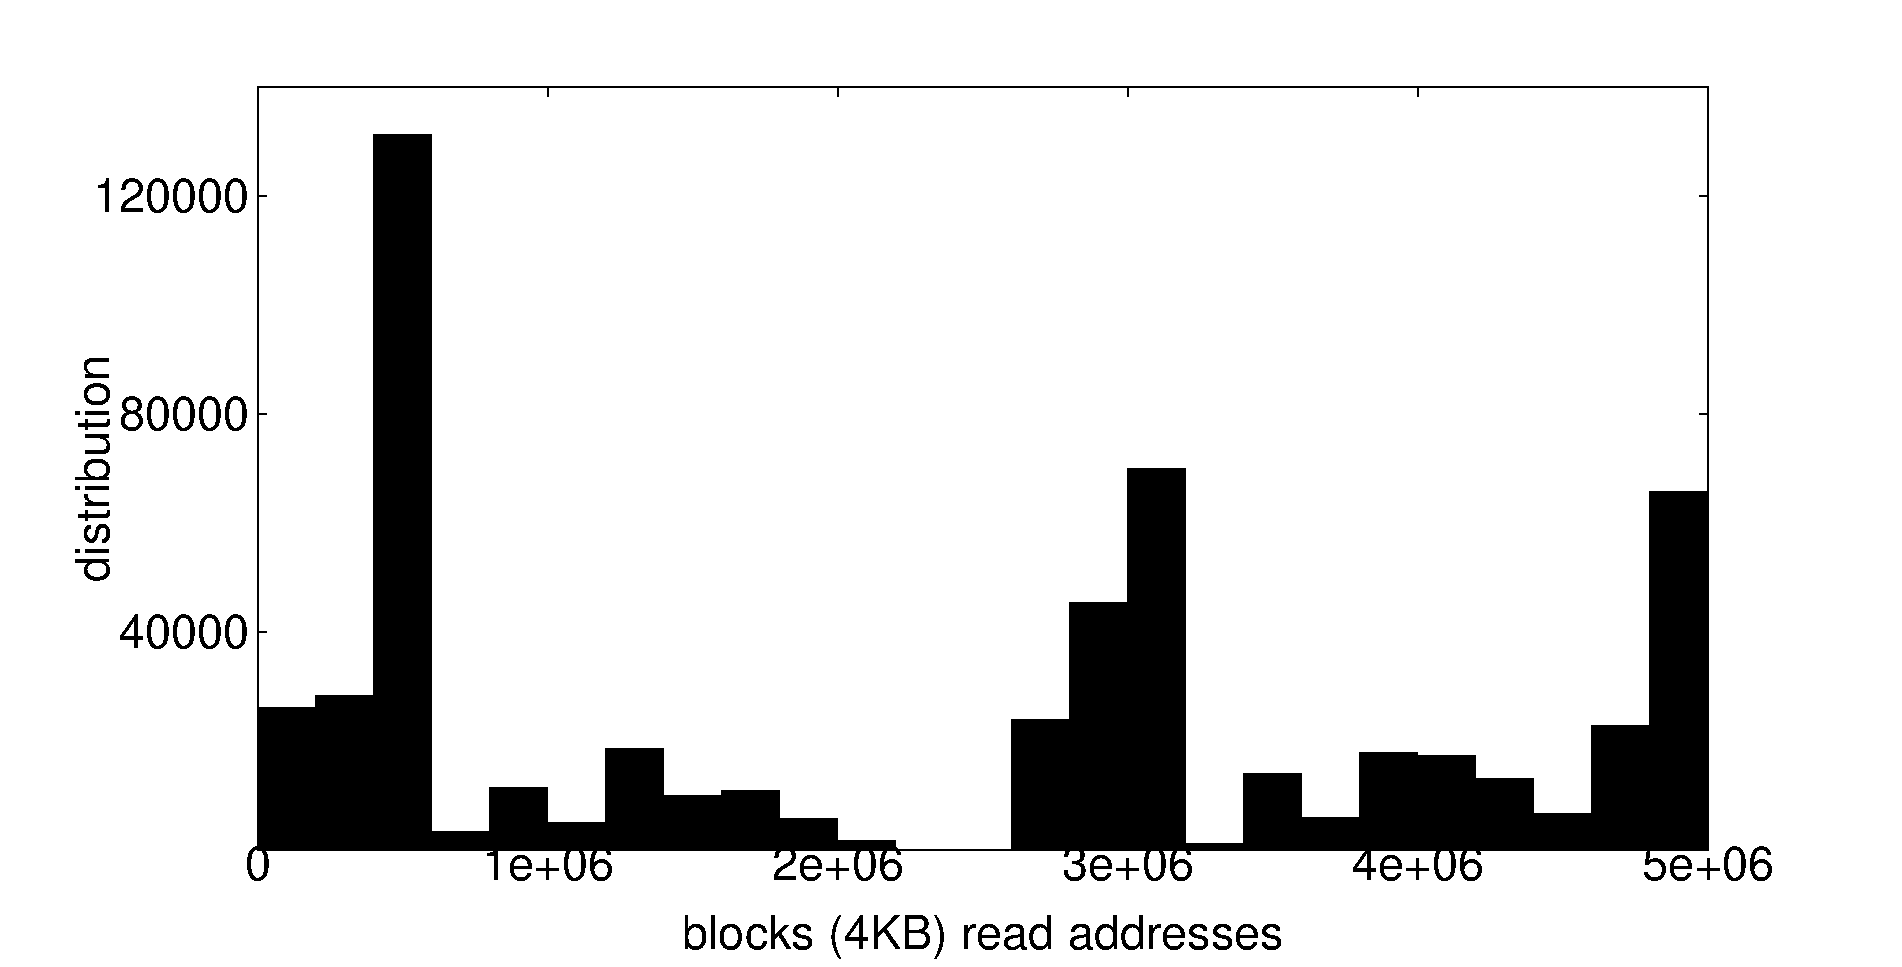
\includegraphics[width=\textwidth]{tracechar-figures/3-day/webvm-block-read-appended-3.eps}
%	\label{fig:webvm-block-read-distrib}
%	\caption{Distribution of blocks read}
%\end{figure}
%\end{minipage} 
%\hfill
%\begin{minipage}[t]{0.6\textwidth}
%\begin{figure}
%	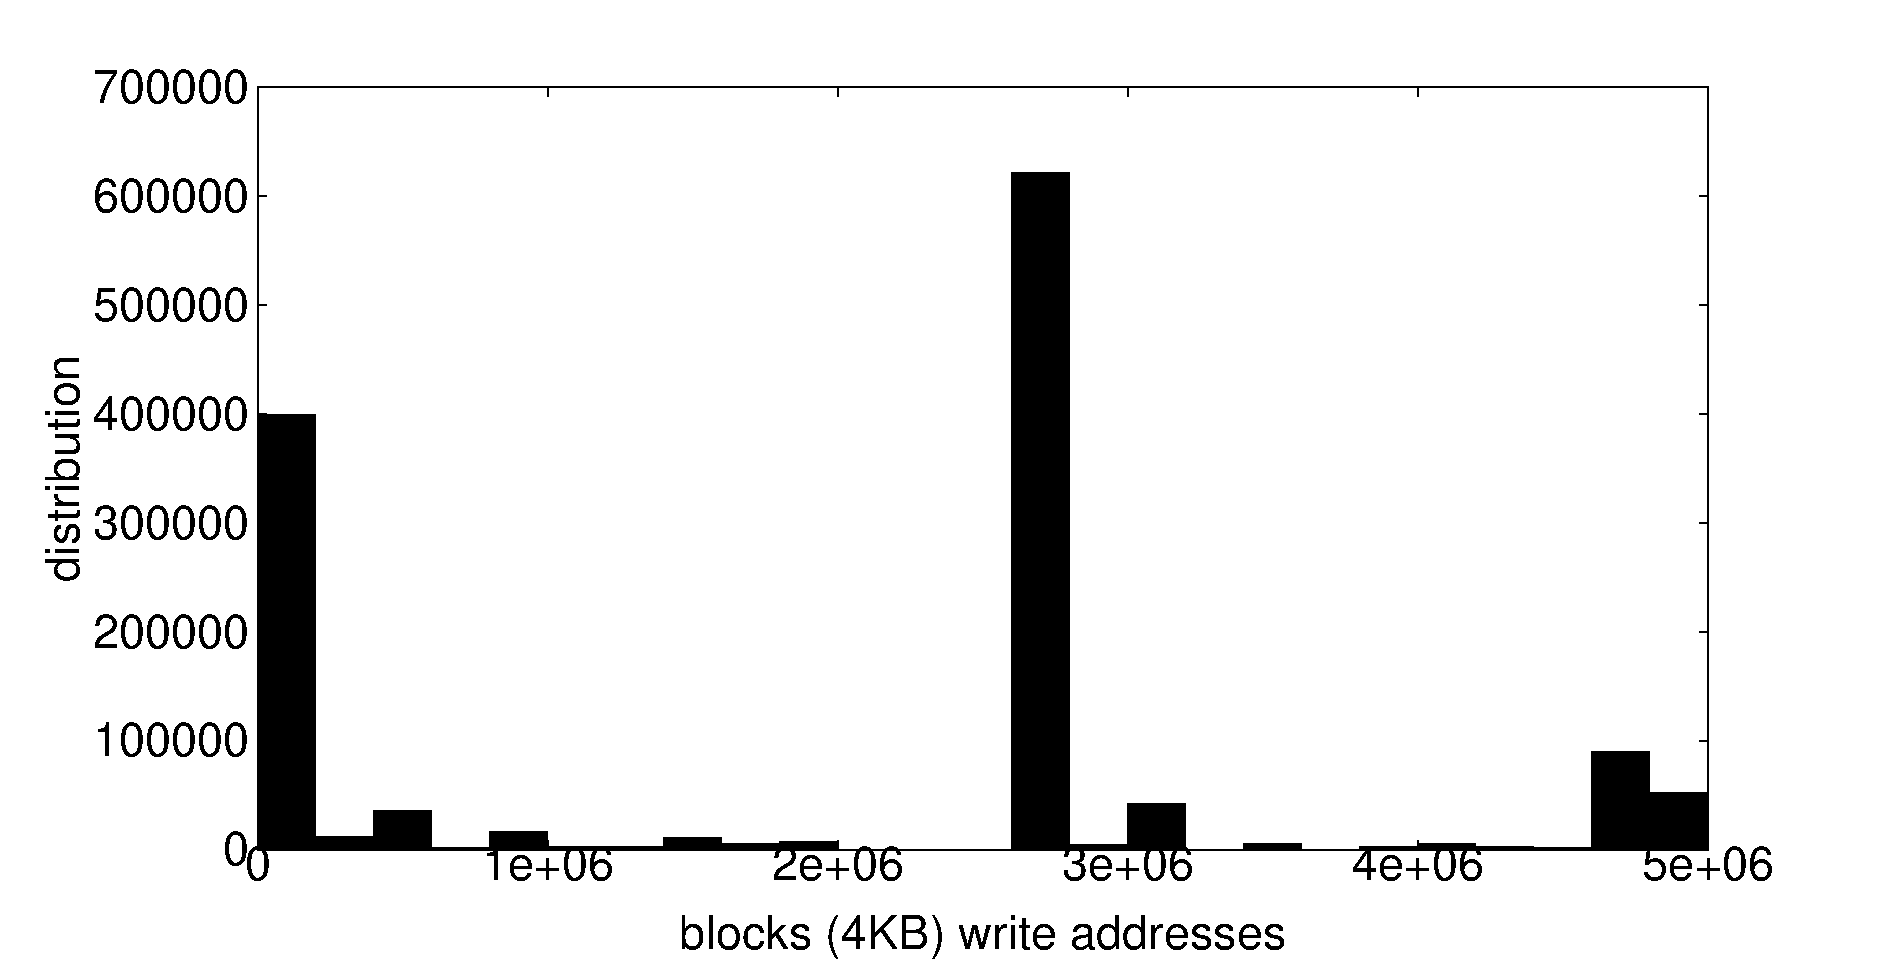
\includegraphics[width=\textwidth]{tracechar-figures/3-day/webvm-block-write-appended-3.eps}
%	\label{fig:webvm-block-write-distrib}
%	\caption{Distribution of blocks written}
%\end{figure}
%\end{minipage}

%\begin{figure*}
%	\centering
%	\vspace{-1.2in}
%	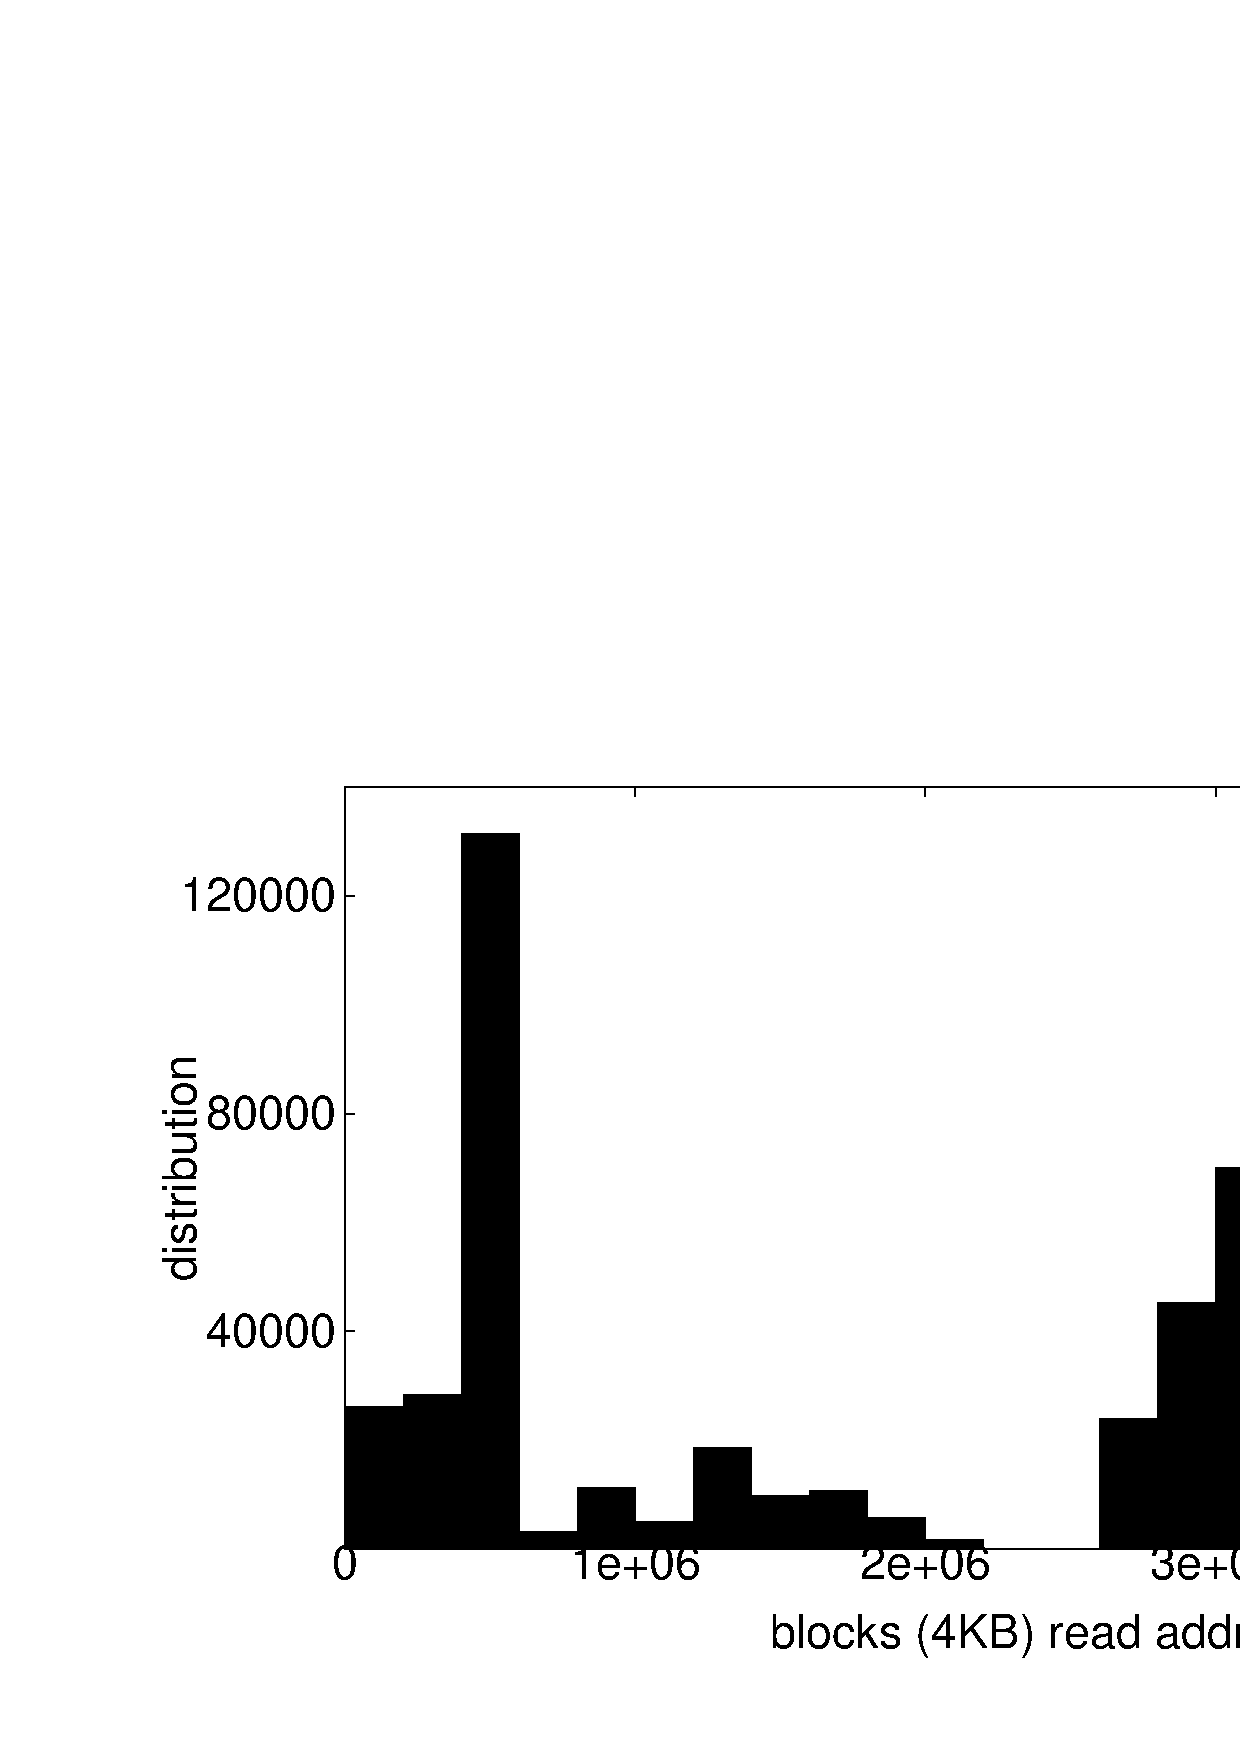
\includegraphics[scale=0.40]{tracechar-figures/3-day/webvm-block-read-appended-3.pdf}
%	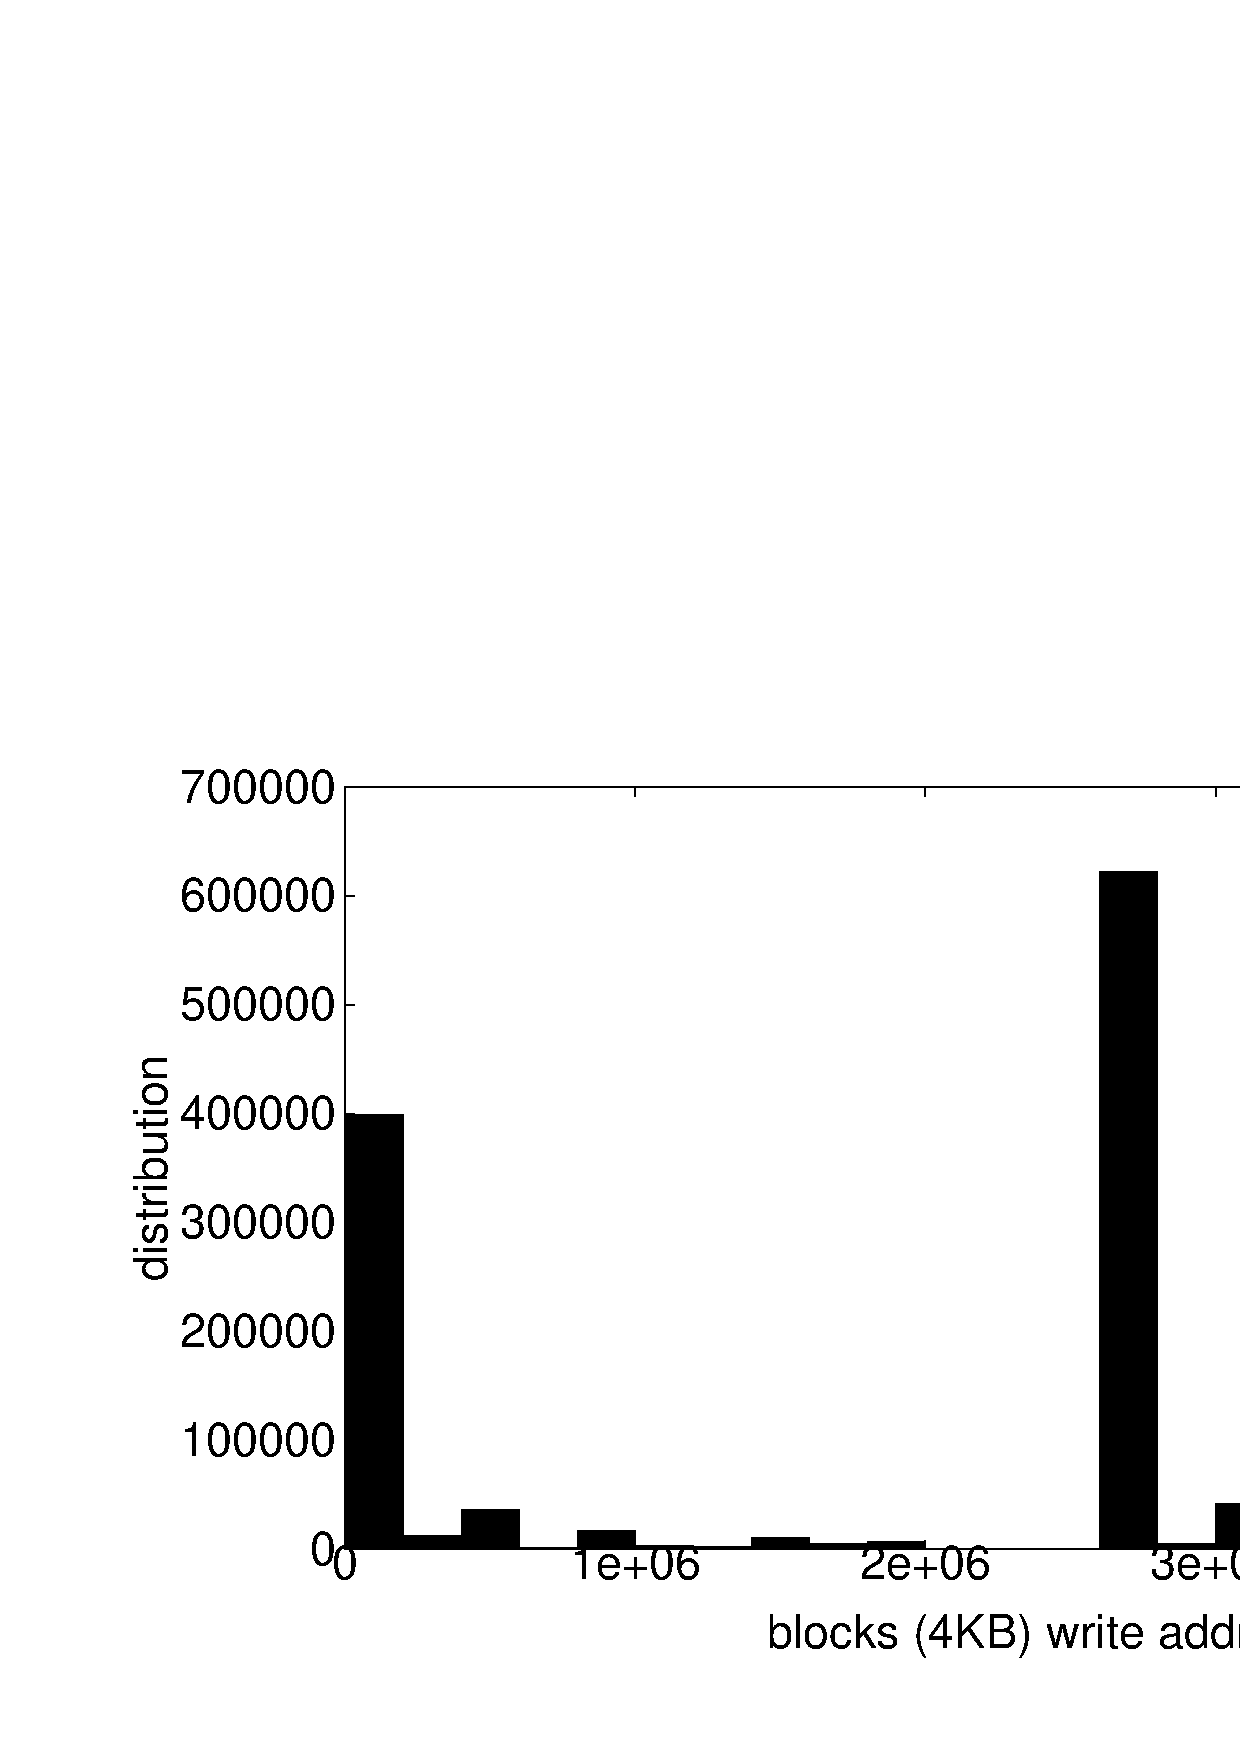
\includegraphics[scale=0.40]{tracechar-figures/3-day/webvm-block-write-appended-3.pdf}
%	\vspace{-1.2in}
%	\caption{Distribution of blocks read and written for the \textit{webvm} trace}
%	\label{fig:webvm-blocks-read-distrib}
%\end{figure*}

Fig.~\ref{fig:webvm-blocks-read-write-distrib}(a) presents a probability distribution 
of the 4KB block addresses read in the \textit{webvm} trace, 
while Fig.~\ref{fig:webvm-blocks-read-write-distrib}(c) presents the same
for the \textit{homes} trace. The x-axis plots the addresses of the blocks 
read or written, respectively, such that each address is for a 4 KB block 
or 8 sectors or 4096 bytes. 
It can be seen that a major portion of
the read accesses in both traces are limited to only some portions of the address space, 
while the rest of the address space gets much fewer read accesses. 
Similar behaviour is observed in the write accesses as well, as shown
in Fig.~\ref{fig:webvm-blocks-read-write-distrib}(b)
and Fig.~\ref{fig:webvm-blocks-read-write-distrib}(d), respectively. 
% Note that, though the
% x-axis limits are the same for both the read and write graphs, the y-axis ranges 
% are different\textemdash{}this is in line with the fact that the total number
% of reads in both the traces is lower than the number of writes.
Note that, the total range of blocks accessed is bigger in case of
the \textit{homes} trace as compared to the \textit{webvm} trace\textemdash{}this is
because the file system size in case of the former is around an order
larger than the latter, as shown in 
Table~\ref{tab:tracechar-summary-stats}.

The above block accessed distributions prove that there is \textit{spatial locality} in
the blocks being accessed in the traces, i.e., the accesses tend to be clustered more
in particular regions instead of being uniformly distributed throughout the address
range. This behaviour is typical of most storage I/O workloads and several
models have been proposed in literature to capture this characteristic
into realistic benchmarks~\cite{jump-based-synthetic, storagecharacterization, storagemodeling,
storagereplay}.

Fig.~\ref{fig:webvm-blocks-read-write-distrib} refers to all (i.e., unique as well as
duplicate) blocks
being accessed in the trace, however since we are interested in I/O
deduplication, it would be interesting to know whether such spatial 
locality of access exists for duplicate data as well. The work in
\cite{idedup} certainly demonstrates this to be true of real-world storage content,
however the question that faces us is whether this is true of I/O workloads 
as well.
\begin{figure}
	\centering
	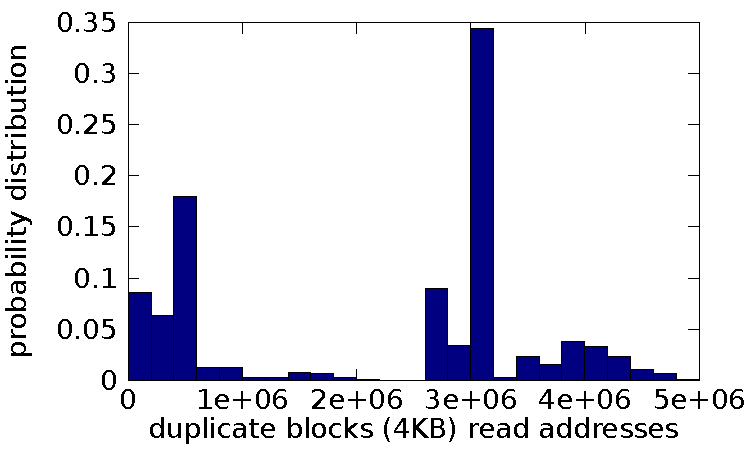
\includegraphics[scale=0.6]{tracechar-figures/21-day/webvm-dedup-block-read-appended-21-prob.pdf}
	\caption{Distribution of accesses of duplicate content blocks}
	\label{fig:webvm-blocks-dedup-distrib}
\end{figure}


To answer the question of spatial locality in duplicate content, we 
consider only those records from the trace which read ``duplicate''
data, i.e., each trace record considered in this scenario is associated
with content that has already been read or written in a previous trace
record. For every block of content that we encounter in the trace, we
assign it an index called the \texttt{dedupID} and if a content is
repeated, it is assigned the same \texttt{dedupID} as the previous
instance of that content in the trace. Thus, \texttt{dedupID} is a
unique identifier for block content, and in 
Fig.~\ref{fig:webvm-blocks-dedup-distrib}
we plot the access distribution for only those content which were 
found to be duplicate in the \textit{webvm} trace.
As expected, we can see in Fig.~\ref{fig:webvm-blocks-dedup-distrib}
that there is spatial locality within the accesses
of duplicate data as well. 
Thus, our observations echo those present in \cite{idedup}.

% Below reasoning based on WRONG input... had accidentally thought that rw=1! meant write...
% However, note that the number of duplicate 
% content instances seems to be much smaller compared to the total number
% of blocks read. Given this observation, one would wonder
% how DRIVE system is able to achieve the significant performance improvement 
% that we observed in Section~\ref{sec:drivechap-experimental-eval}. The
% reason is that DRIVE evaluation was performed over the entire three 
% week long trace, whereas these distributions have been presented only for
% the trace of the first 3 days therein. This trace snippet has 
% around 550K (556539) reads and 1300K (1328233) writes, giving a total
% of around 1850K (1884772) block trace records.

% As can be seen in 
% Fig~\ref{fig:contentdedup-factor-timeseries} of 
% Section~\ref{sec:drivechap-experimental-eval},
% the content deduplication in DRIVE system really starts performing
% significantly well
% only much later during the trace replay. This indicates that the 
% \textit{webvm} trace most likely has higher levels of duplicate content
% access in the later days' traces than the earlier days. This further
% hints that using small synthetic benchmarks is unlikely to prove DRIVE's
% performance benefits, as opposed to evaluation on realistic 
% long-running benchmarks.

\subsection{Run length distribution}
In general, run length refers to the length of a sequential run. In the
context of I/O traces, \textit{run length} refers to the length of 
a sequence of blocks being requested. For example, if the block accesses
occur as shown in Fig.~\ref{fig:runlength-example}, the first sequence
of block accesses results in a run length of 3, the second sequence has
a run length of 5, and the third sequence has a run length of 1. 

\begin{figure}
	\centering
	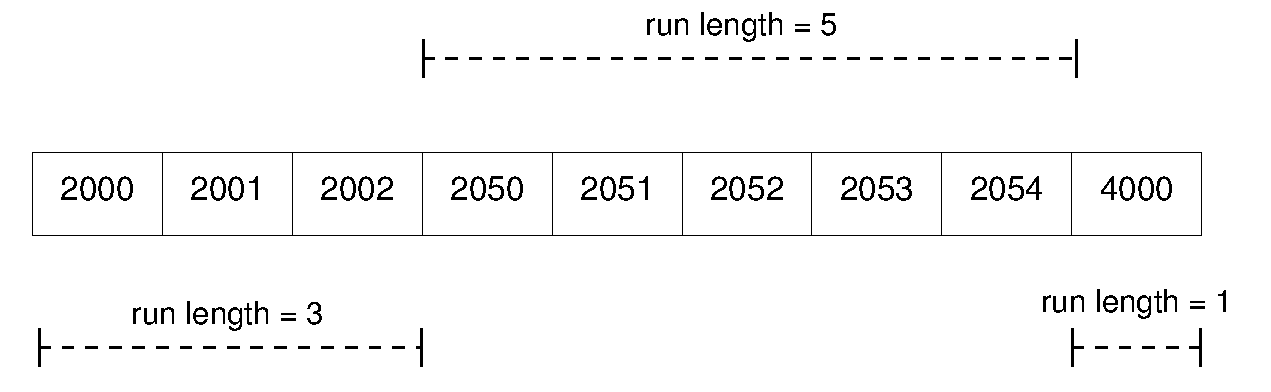
\includegraphics[scale=0.55]{tracechar-figures/21-day/runlength-example.pdf}
	\caption{Example to explain the definition of \textit{run length}}
	\label{fig:runlength-example}
\end{figure}

For \textit{webvm} trace characterization, we present its run length
distribution, i.e., a distribution of the different length sequences
in the trace. This metric will indicate whether requests in the
trace have the sequentiality property, or whether they are essentially
random access. It may be noted that if there are many huge files being
accessed or read from the file system, it will cause bigger run lengths
to be recorded in the trace. On the other hand, if the files being read are 
small (i.e. less than 4KB in size), then the read workload will seem to be
random instead of sequential, since entire files
each will get read in a single I/O~\cite{animation-nfs}.

\begin{figure}[t]
	\centering
	\subfloat[Block run length for reads (\textit{webvm})]{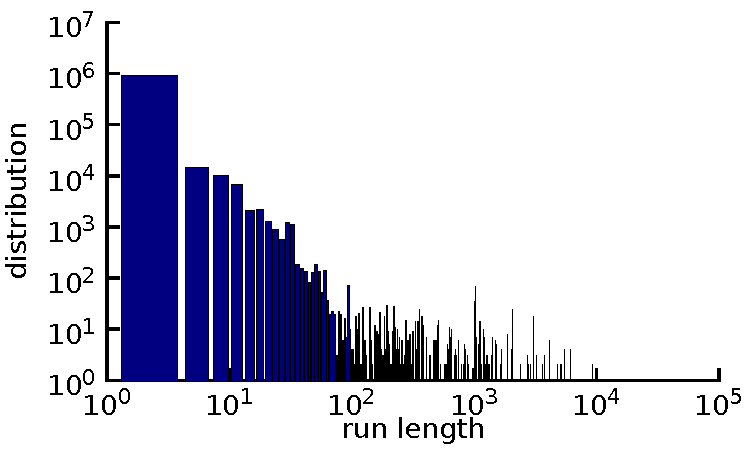
\includegraphics[scale=0.6]{tracechar-figures/21-day/webvm-run-length-distrib-readonly-appended-21-loglog.pdf}} 
	\hfill
	\subfloat[Block run length for writes (\textit{webvm})]{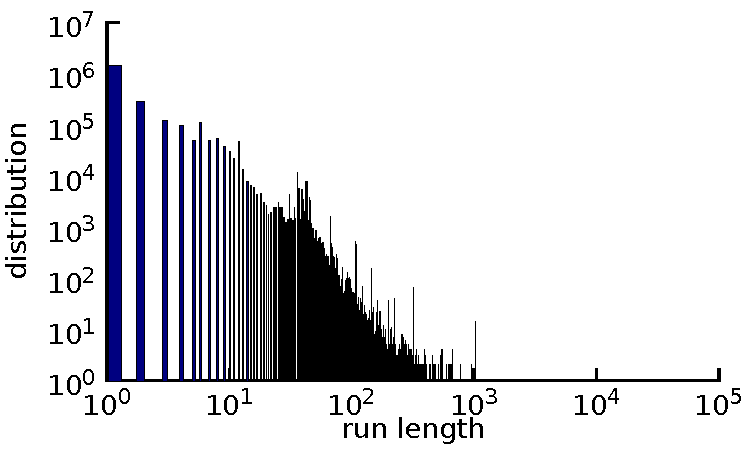
\includegraphics[scale=0.6]{tracechar-figures/21-day/webvm-run-length-distrib-writeonly-appended-21-loglog.pdf}}
	\\
	\subfloat[Block run length for reads (\textit{homes})]{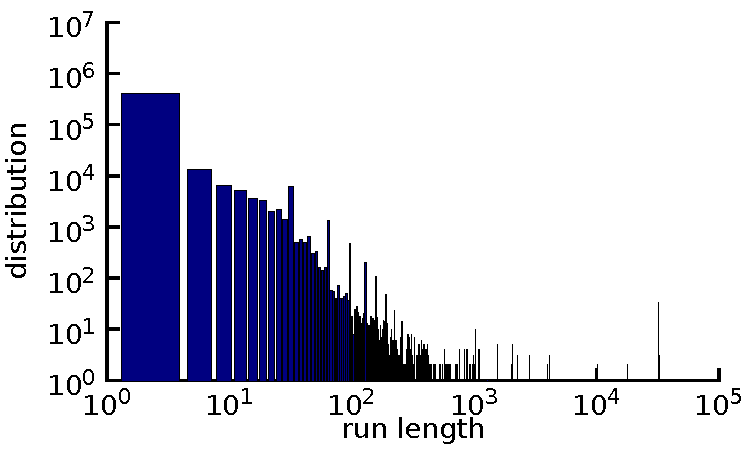
\includegraphics[scale=0.6]{tracechar-figures/21-day/homes-run-length-distrib-readonly-appended-21-loglog.pdf}} 
	\hfill
	\subfloat[Block run length for writes (\textit{homes})]{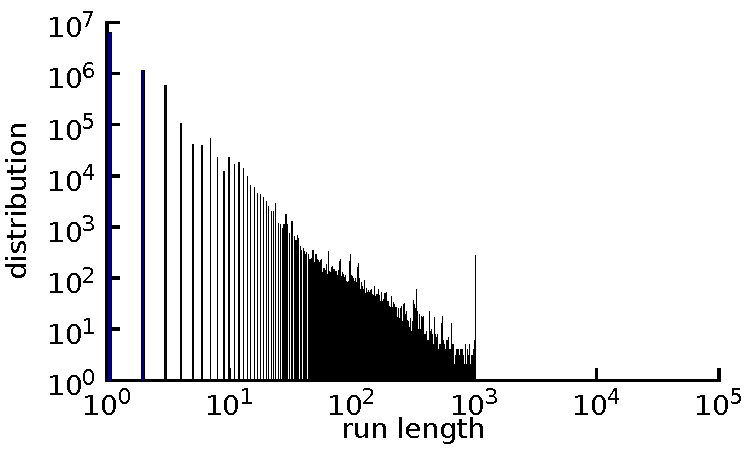
\includegraphics[scale=0.6]{tracechar-figures/21-day/homes-run-length-distrib-writeonly-appended-21-loglog.pdf}}
	\caption{\textit{Block run length} distribution for reads and writes in \textit{webvm} and \textit{homes} traces}
	\label{fig:webvm-runlength-read-write-distrib}
\end{figure}



%\begin{figure}[t]
%	\centering
%	\subfloat[Run length for duplicate content blocks accessed consecutively]{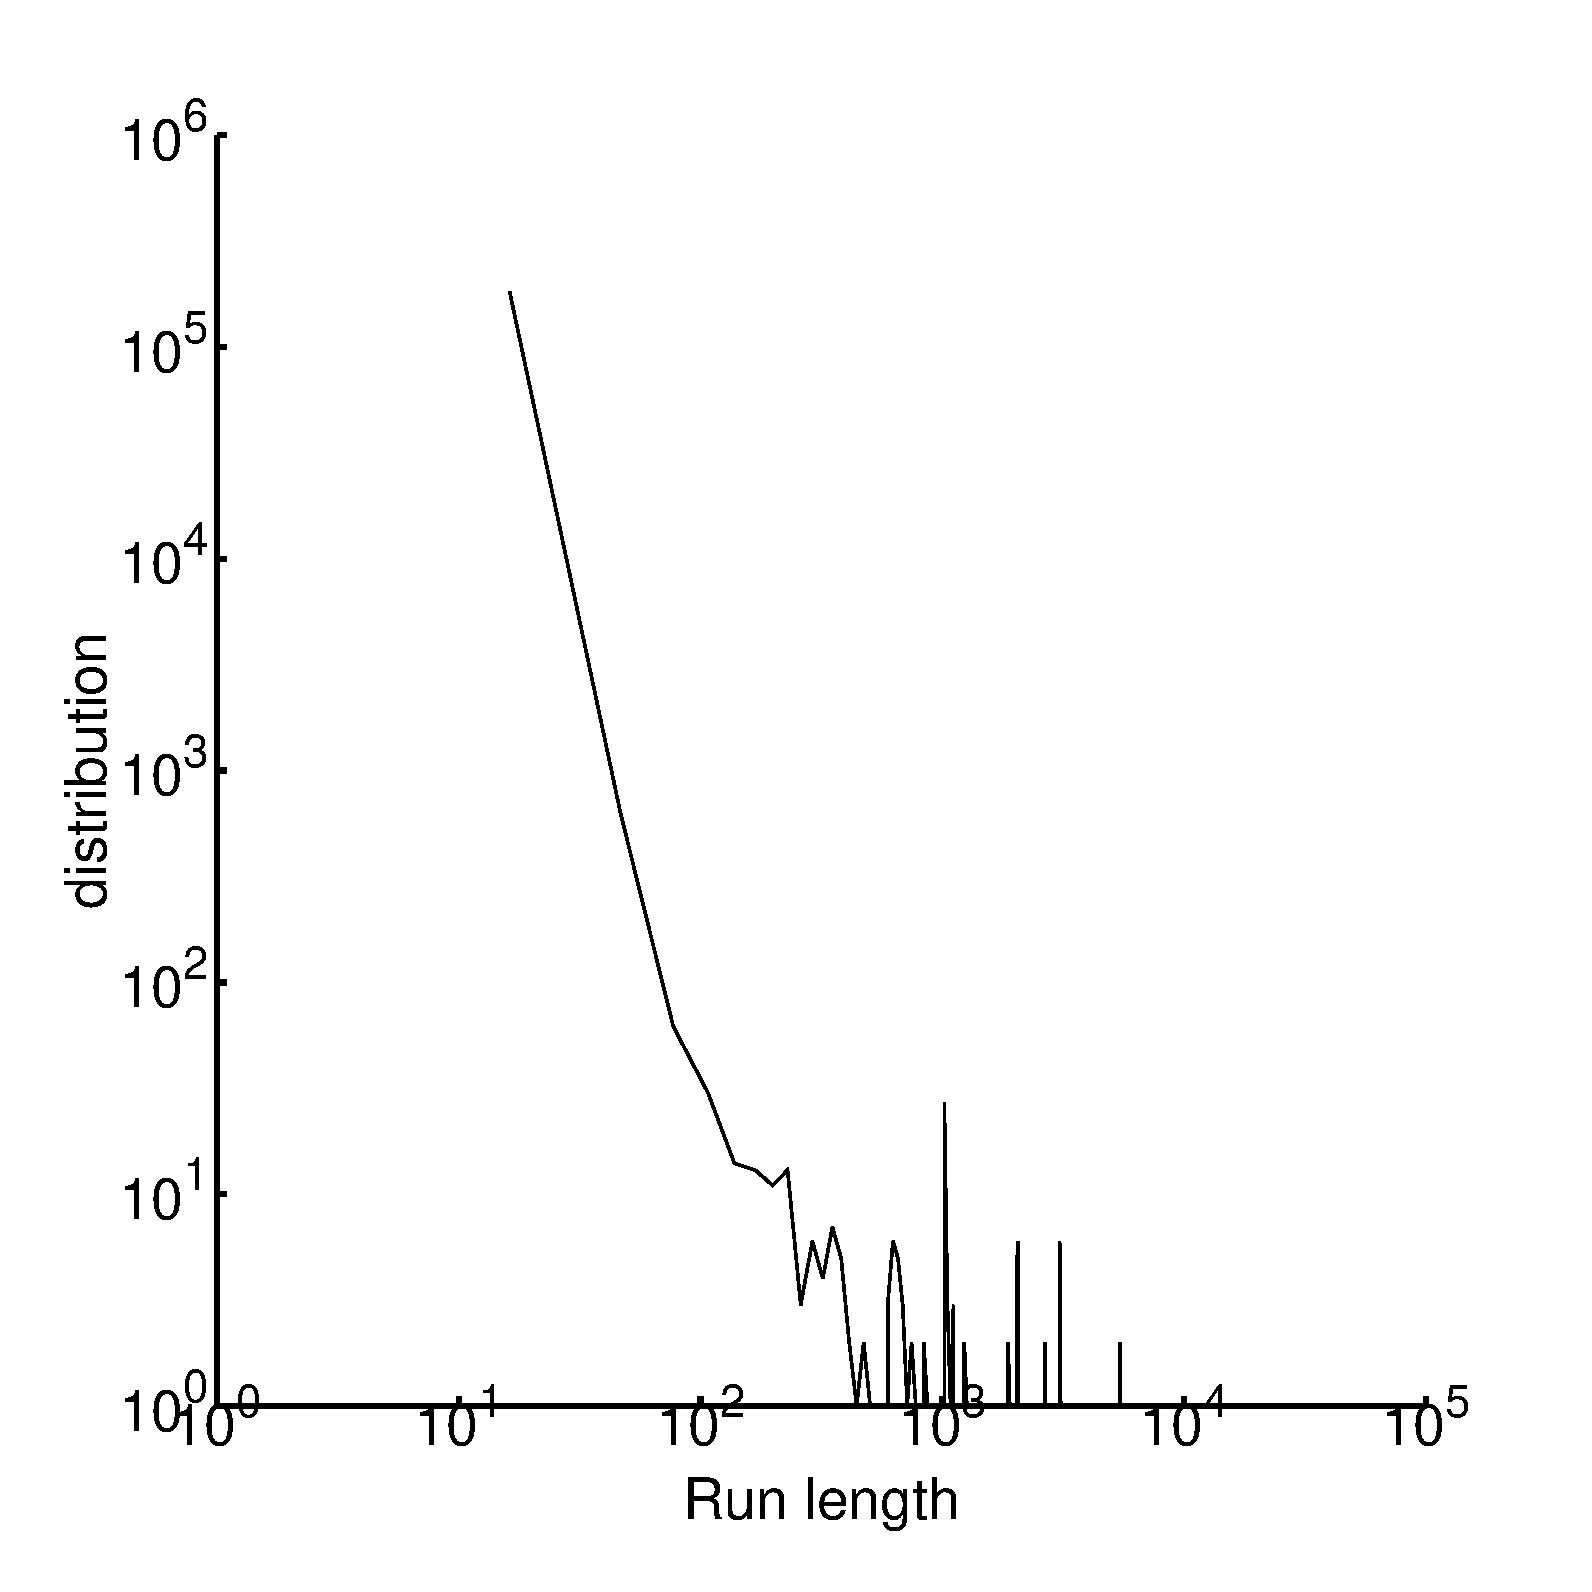
\includegraphics[scale=0.4]{tracechar-figures/3-day/webvm-run-length-distrib-readonly-appended-3-loglog.eps}}
%	\label{fig:webvm-runlength-read-write-distrib}
%\end{figure}

The run length distributions for read and write requests have been 
plotted in Fig.~\ref{fig:webvm-runlength-read-write-distrib}, where it
can be seen that as the run length increases, the number of occurrences
of that run length reduces. More specifically, read request run length
distribution for \textit{webvm} and \textit{homes} reveals
the following important points:-
\begin{enumerate}

	\item Read run length of less than 10 blocks occur close to $10^6$
		times in both \textit{webvm} and \textit{homes} traces
	\item Read run length of between 10 to 100 blocks occur between
		10 to $10^4$ times in both traces
	\item Read run length of greater than 100 blocks occur around 10 times or less
\end{enumerate}
The above observations enable us to conclude that very long run lengths 
in read I/O are rare whereas run length of less than 10 blocks is mostly 
the norm. Our observation of 82\% run lengths being of 1 block also 
corroborates the finding in \cite{storagecharacterization} that most I/O 
in web service applications is found to be random access and not sequential.

The write request run length distribution plotted in 
Fig.~\ref{fig:webvm-runlength-read-write-distrib}(b) 
shows that a similar characteristic (as observed
with reads) is present here as well. The following points may be noted:-
\begin{enumerate}
	\item In both cases, there is a huge number of instances of run length = 1
	\item The maximum write run length is only around 3$\times 10^3$ whereas 
		the maximum read run length is over a magnitude larger at around
		3$\times 10^4$
	\item The maximum run length for reads in \textit{homes} trace is 32,510 blocks compared
      to 1024 blocks for write run length		
\end{enumerate}

To achieve a better comparison across these different plots, we present the
probability distributions below
in Fig.~\ref{fig:runlength-read-write-distrib-prob}, such that the total number of requests 
within the trace doesn't skew the number of instances in each bucket.
In fact, the probability distribution captures which is the most expected
and least expected run length in each of the considered cases.
From Fig.~\ref{fig:runlength-read-write-distrib-prob}, we can see that
\begin{enumerate}
 \item The number of instances of run length = 1 in case of read requests in \textit{webvm}
		trace is proportionally much higher than the corresponding write requests, 
		specifically 86\% in reads as opposed to 57\% in writes
 \item 75\% of the values in the both the read and write run 
      length distribution of \textit{homes} trace are for run length = 1 block
 \item Additionally, the read requests of both the \textit{webvm} and \textit{homes} trace
      have more instances
      of run length less than 10, as compared to the write requests
\end{enumerate}
From the above, we can conclude that, in both the \textit{webvm} and \textit{homes} traces,
read run lengths are generally shorter than write lengths, which is indicated
by the read run length distributions having taller bars for shorter run lengths,
and shorter bars for longer run lengths, in comparison to the write run length
distributions.



%block numbers accessed consecutively, and duplicate content blocks accessed consecutively
\begin{figure}[t]
	\centering
	\subfloat[Block run length for reads (\textit{webvm})]{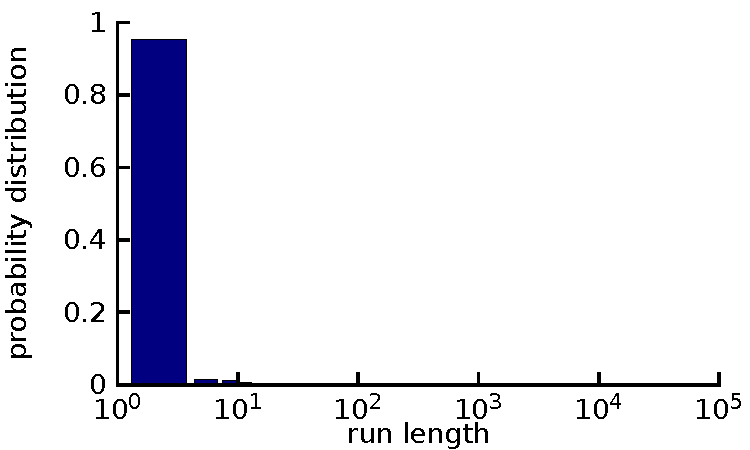
\includegraphics[scale=0.6]{tracechar-figures/21-day/webvm-run-length-distrib-readonly-appended-21-prob.pdf}} 
	\hfill
	\subfloat[Block run length for writes (\textit{webvm})]{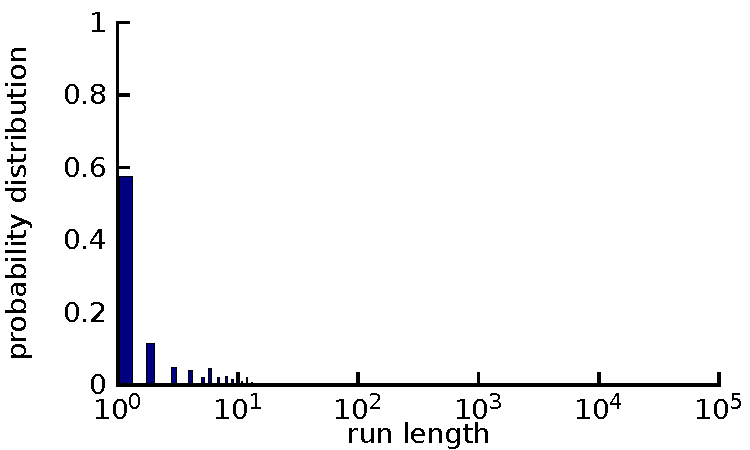
\includegraphics[scale=0.6]{tracechar-figures/21-day/webvm-run-length-distrib-writeonly-appended-21-prob.pdf}}
	\\
	\subfloat[Block run length for reads (\textit{homes})]{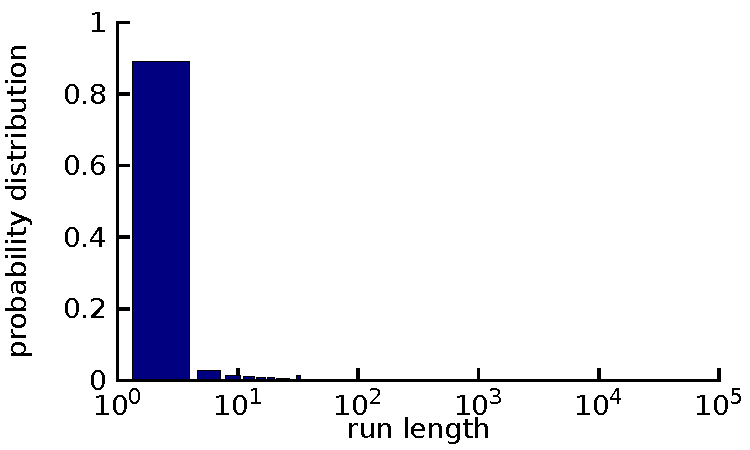
\includegraphics[scale=0.6]{tracechar-figures/21-day/homes-run-length-distrib-readonly-appended-21-prob.pdf}} 
	\hfill
	\subfloat[Block run length for writes (\textit{homes})]{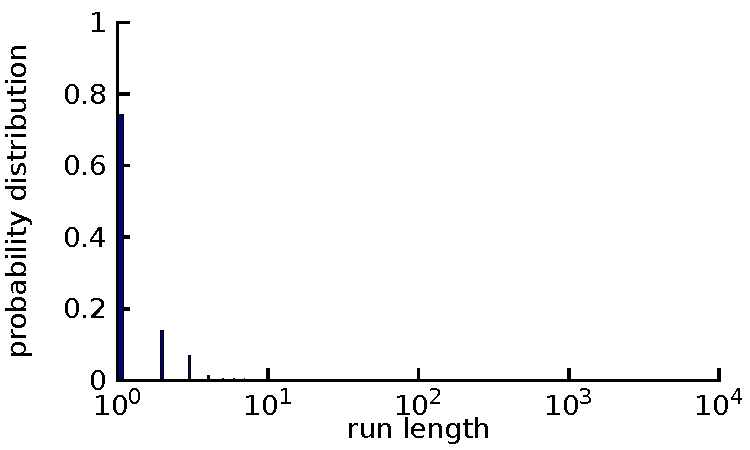
\includegraphics[scale=0.6]{tracechar-figures/21-day/homes-run-length-distrib-writeonly-appended-21-prob.pdf}}
	\caption{\textit{Block run length} probability distribution for reads and writes in \textit{webvm} and \textit{homes} traces}
	\label{fig:runlength-read-write-distrib-prob}
\end{figure}


  
Since our study is geared towards understanding the duplicate content
characteristics of the trace, we further present a content-defined version
of the \textit{run length} metric, which we refer to as the 
\textit{duplicate content run length}. Basically, this metric tries to
capture whether the duplicate content blocks are those that have a run
length of one, or those with longer run lengths.
% , which has further
% implications on whether data access patterns will get fragmented or not 
% due to I/O deduplication. 

By investigating the \textit{duplicate content run length} metric, we
observed that \textbf{all} the 158852 read requests that were found to
have duplicate content in \textit{webvm} trace were of run length = 1 block.
% within the original trace. 
% Thus, we observe that none of the sequences
% with run length greater than 1 got deduplicated.
This is understandable, since most of the read requests in the trace 
were of run length = 1 block as well (86\% as reported above).
% This also shows that there is
% no risk of I/O causing a random access pattern, because the access pattern
% is random even without the I/O deduplication optimization.

%\begin{figure}
%	\centering
%	\includegraphics[scale=0.4]{tracechar-figures/3-day/webvm-dedup-run-length-read-appended-21.eps}
%	\label{fig:webvm-run-length-dedup-distrib}
%	\caption{Distribution of duplicate content run length}
%	\vspace{-0.2in}
%\end{figure}



\subsection{Reuse distance distribution}

\begin{figure}
	\centering
	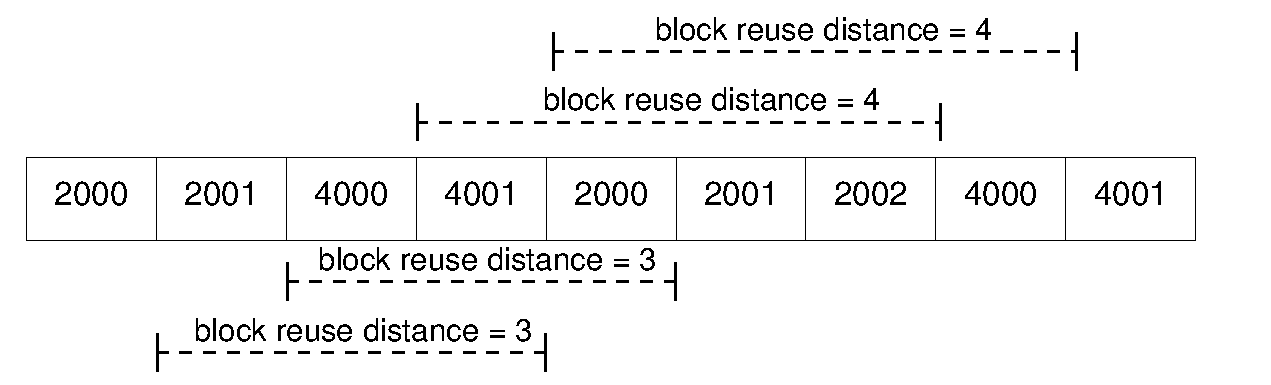
\includegraphics[scale=0.6]{tracechar-figures/21-day/reusedist-example.pdf}
	\caption{Example to explain the definition of \textit{block reuse distance}}
	\label{fig:reusedist-example}
\end{figure}

The term \textit{reuse distance} refers to the number of blocks (or content)
between two successive accesses to the same block (or content)~\cite{iodedup}. 
An example of block reuse distance is
presented in Fig.~\ref{fig:reusedist-example} which shows a series
of blocks\textemdash{}2000, 2001, 4000, 4001, 2000, 2001, 2002, 4000, 4001\textemdash{}being
accessed. In this sequence, the blocks 2000, 2001, 4000 and 4001 have
been ``reused'', i.e., accessed more than once. The reuse distance in
each of these cases is as marked in the figure, i.e. reuse distance
= 3, 3, 4, 4, respectively. Similarly, \textit{content reuse distance}
is defined per access of same content, and is irrespective of its block 
address. Thus, if blocks 2000 and 4000 have duplicate content as shown
in Fig.~\ref{fig:content-reusedist-example}, then content reuse distances
for that content would be 1, 1 and 2 in the given example.

A study of \textit{block reuse distance} versus \textit{content reuse distance}
for the \textit{webvm} trace is present in \cite{iodedup}, however only
``average'' distances are reported whereas we present the ``distribution'' here.
Similar to the observation in \cite{commercial-characterization}, we also
believe that distributions paint a better picture of the overall scenario
than mere averages.


\begin{figure}
	\centering
	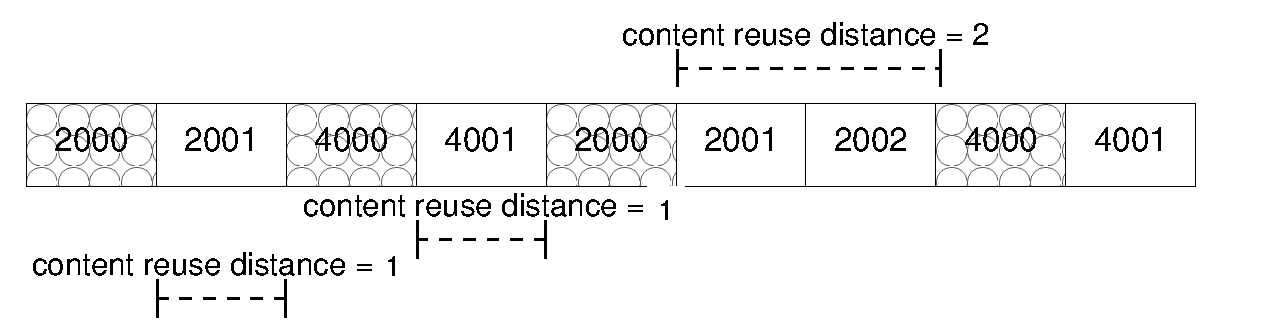
\includegraphics[scale=0.6]{tracechar-figures/21-day/content-reusedist-example-fixedmanual-2.pdf}
	\caption{Example to explain the definition of \textit{content reuse distance}}
	\label{fig:content-reusedist-example}
\end{figure}

\begin{figure}[t]
	\centering
	\subfloat[Read blocks (\textit{webvm})]{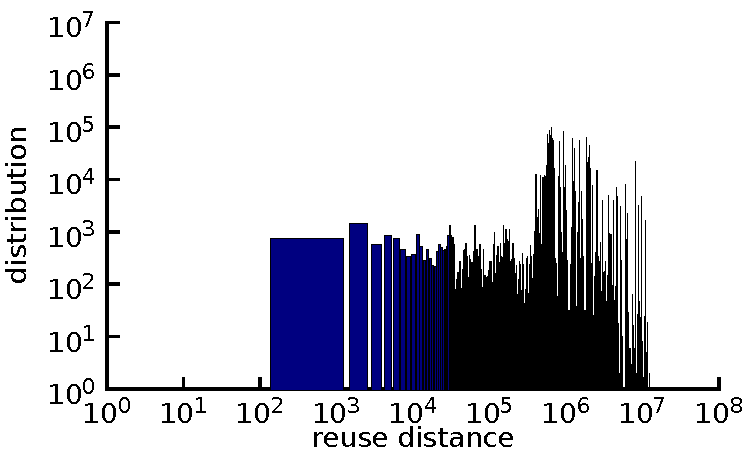
\includegraphics[scale=0.6]{tracechar-figures/21-day/webvm-reuse-dist-distrib-readonly-appended-21-loglog.pdf}} \hfill
	\subfloat[Write blocks (\textit{webvm})]{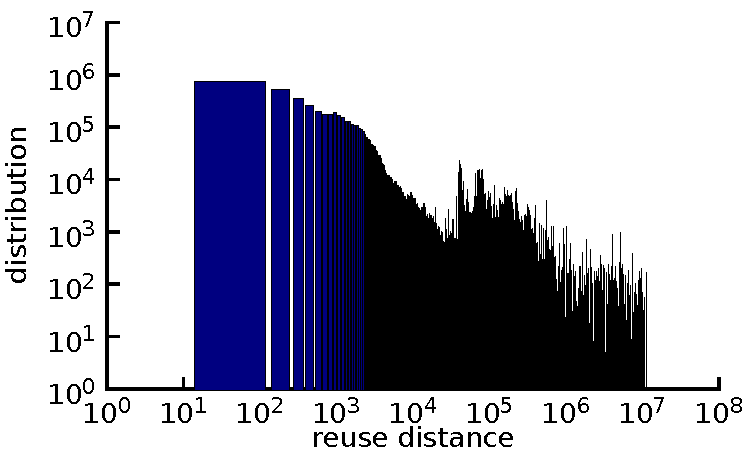
\includegraphics[scale=0.6]{tracechar-figures/21-day/webvm-reuse-dist-distrib-writeonly-appended-21-loglog.pdf}}
	\\
	\subfloat[Read blocks (\textit{homes})]{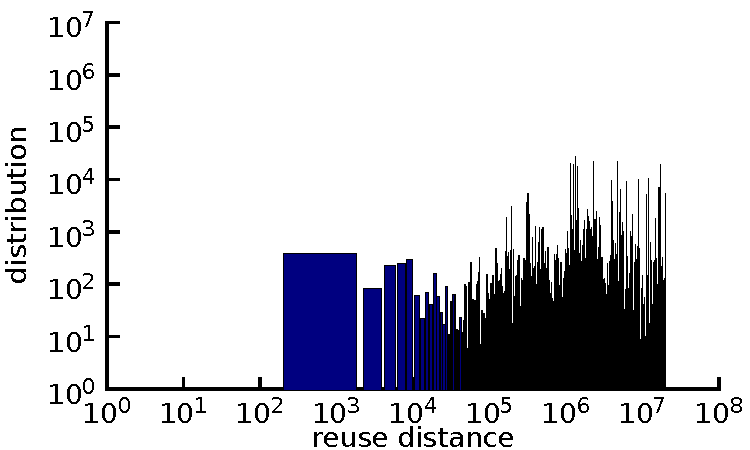
\includegraphics[scale=0.6]{tracechar-figures/21-day/homes-reuse-dist-distrib-readonly-appended-21-loglog.pdf}} \hfill
	\subfloat[Write blocks (\textit{homes})]{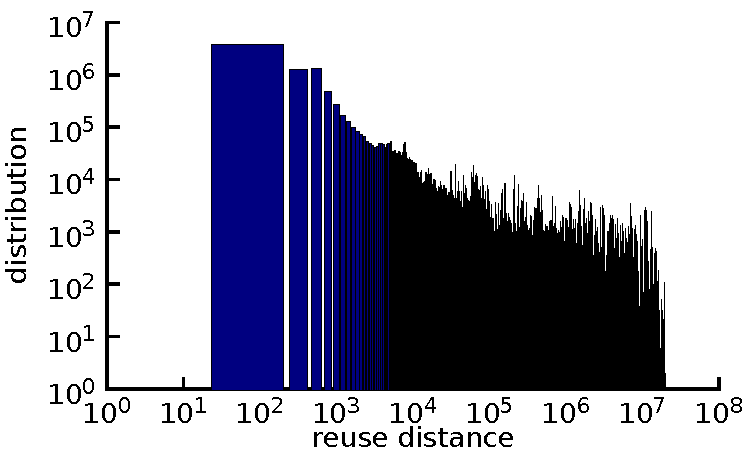
\includegraphics[scale=0.6]{tracechar-figures/21-day/homes-reuse-dist-distrib-writeonly-appended-21-loglog.pdf}}	
	\caption{\textit{Block reuse} distance distribution for reads and writes in \textit{webvm} and \textit{homes} traces}
	\label{fig:reusedist-read-write-distrib}
\end{figure}

The block reuse distance distributions for the read and write requests for
both the \textit{webvm} and the \textit{homes} traces are plotted in
Fig.~\ref{fig:reusedist-read-write-distrib}. 
In both read and write distributions, \textit{webvm} trace has greater occurrence of
smaller reuse distances that the \textit{homes} trace. Also, both traces have 
smaller reuse distances for write requests as compared to read requests. This 
may be because when files are over-written using an editor, its corresponding
blocks that have been fetched into page cache, tend to get freed up and new
blocks allocated for writing the new content~\cite{longterm-fair}. 
The blocks that get freed up thereby, might get re-allocated soon as and when
new write requests come in\textemdash{}this may result in a higher churn of write blocks, 
in write-intensive workloads.


\begin{figure}[t]
	\centering
	\subfloat[Read content (\textit{webvm})]{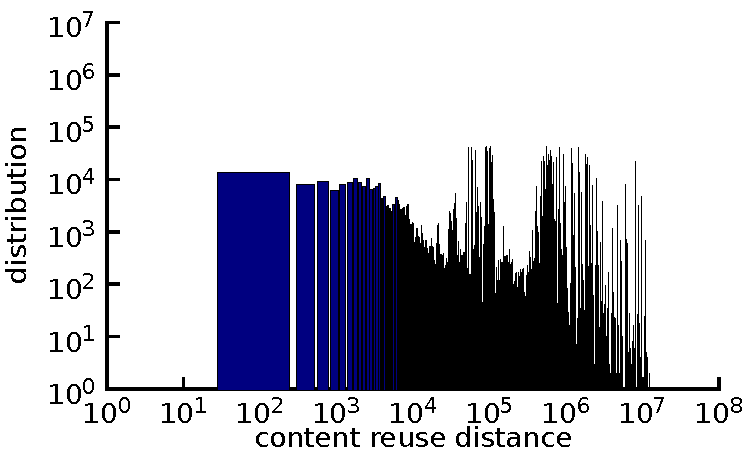
\includegraphics[scale=0.6]{tracechar-figures/21-day/webvm-reuse-dist-distrib-dedup-readonly-appended-21-loglog.pdf}} \hfill
	\subfloat[Write content (\textit{webvm})]{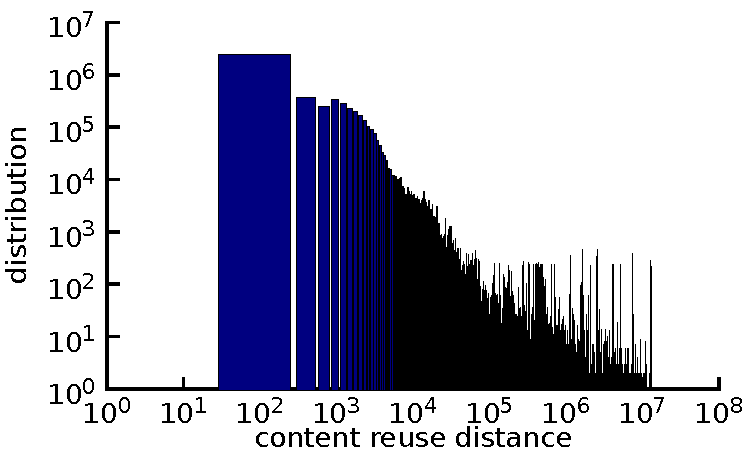
\includegraphics[scale=0.6]{tracechar-figures/21-day/webvm-reuse-dist-distrib-dedup-writeonly-appended-21-loglog.pdf}}
	\\
	\subfloat[Read content (\textit{homes})]{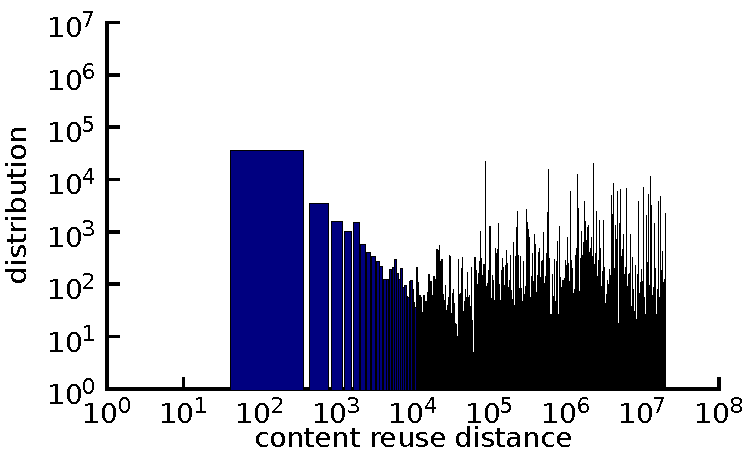
\includegraphics[scale=0.6]{tracechar-figures/21-day/homes-reuse-dist-distrib-dedup-readonly-appended-21-loglog.pdf}} \hfill
	\subfloat[Write content (\textit{homes})]{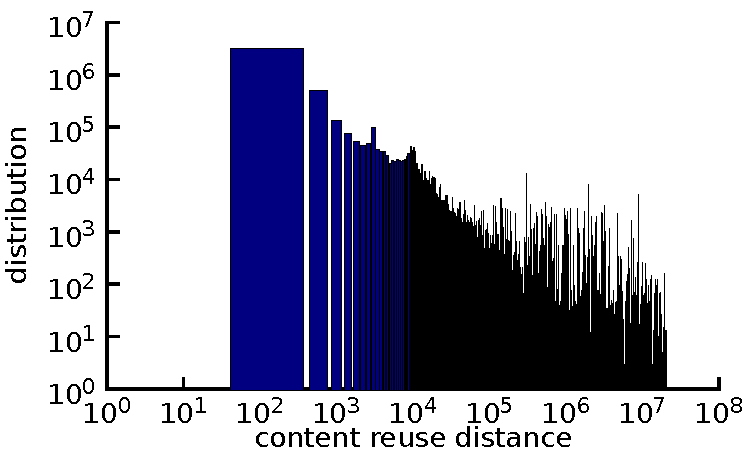
\includegraphics[scale=0.6]{tracechar-figures/21-day/homes-reuse-dist-distrib-dedup-writeonly-appended-21-loglog.pdf}}	
	\caption{\textit{Content reuse} distance distribution for reads and writes in \textit{webvm} trace}
	\label{fig:reusedist-dedup-read-write-distrib}
\end{figure}


As per our observations in Section~\ref{sec:similarity-study} regarding the similarity
study within the three traces, we had concluded that the number of occurrences of
each piece of content was greater than the number of distinct block numbers that
had the same piece of content. In other words, occurrence factor was found to 
be greater than sharing factor for each content. This would imply that the 
distance between accesses to the ``same'' content should be lower than the 
distance between accesses to the same block. To verify this, we present a distribution of 
the content reuse distance in Fig.~\ref{fig:reusedist-dedup-read-write-distrib}.

By comparing each of the graphs Fig.~\ref{fig:reusedist-dedup-read-write-distrib} (a),
(b), (c) and (d) with Fig.~\ref{fig:content-reusedist-example} (a), (b), (c)
and (d), respectively, we can see that in each case, the \textit{content reuse distances}
are smaller than the \textit{block reuse distances}, as expected. Also, the number of
instances of the smallest content reuse distance in each case, is at least an order
of magnitude larger than the number of instances of the smallest block reuse distance,
respectively. Note that, shorter content reuse distance indicates that if the cache
is operated in a content-based manner rather than location-based manner, it would provide
greater benefits~\cite{iodedup}.

\begin{table}[t]
 \caption{Reuse distance statistics for reads in \textit{webvm} and \textit{homes} traces}
%  \hspace{-0.2in}
 \begin{center}
 \begin{tabular}{|c|c|c|c|c|c|} \hline
   \bf{Workload} & \bf{Total} & \bf{Reads with} & \bf{Reads with} & \bf{Reads with} & \bf{Reads with} \\
  \bf{type} & \bf{reads} & \bf{block reuse} & \bf{block reuse} & \bf{content reuse} & \bf{content reuse} \\ 
	    & \bf{(\#)} & \bf{(\#)} & \bf{(\% of total)} & \bf{(\#)} & \bf{(\% of total)} \\ \hline  
  \textit{webvm} & 3,116,456 & 2,800,411 & 90 & 2,873,998 & 92 \\
  \textit{homes} & 4,052,176 & 695,747 & 17 & 732,265  & 18 \\ \hline
 \end{tabular}
 \label{tab:reuse-dist-read-summary}
 \end{center}
 \end{table}
At a high-level view, it may seem that both the \textit{webvm} and \textit{homes}
traces have similar block and content reuse-distance distributions. Note however that,
the axes in these graphs are log-log, so even a ``slight'' difference
can be considered as a significant difference in normal scale. 
To demonstrate that the difference between
them is significant enough to result in differential performance for the two traces, 
we present the statistics in 
Table~\ref{tab:reuse-dist-read-summary} regarding the total number of 
read requests in each trace, and the number of read requests resulting
in block reuse and content reuse in each of them.



\subsection{Jump distance distribution}
In the context of I/O traces, \textit{jump distance} refers to the
distance between successive I/O requests. Specifically, if consecutive
requests are continuous in the logical block address (LBA or LBN) space, 
then the jump distance between them is zero. However, when there are
two consecutive requests (read or write combined) such that they are
not continuous, there is said to be a positive jump distance between
them, equal to the difference between the two block addresses.
Considering the example in Fig.~\ref{fig:jumpdist-example}, we can see
that the given request trace consists of three sequences of 
accesses\textemdash{}2000 to 2002, 2050 to 2054, and 4000. Thus, two non-zero
``jump distances'' can be noted in the example, one after access to
block 2002 and the other after block number 2054.


\begin{figure}
	\centering
	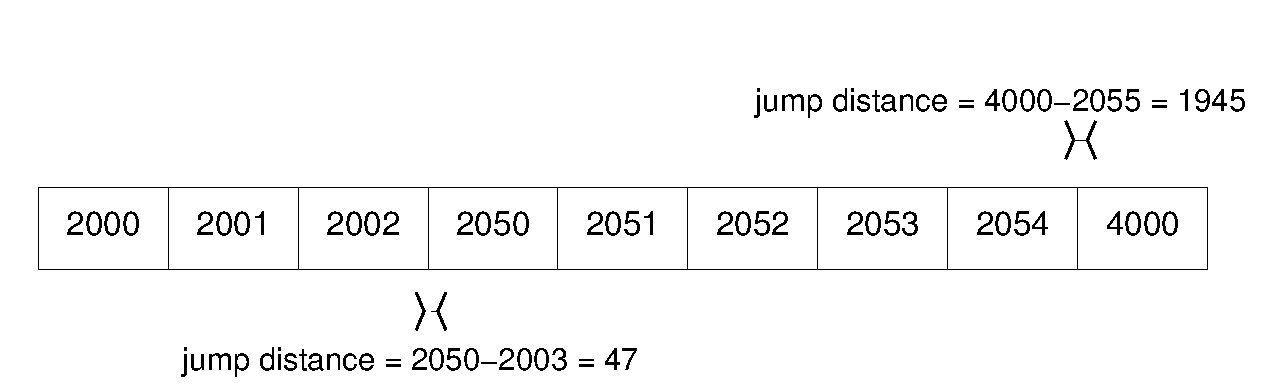
\includegraphics[scale=0.6]{tracechar-figures/21-day/jumpdist-example.pdf}
% 	\vspace{-0.3in}
	\caption{Example to explain the definition of \textit{jump distance}}
	\label{fig:jumpdist-example}
\end{figure}

% \begin{figure}[t]
% 	\centering
% 	\subfloat[Jump distance distribution for block reads]{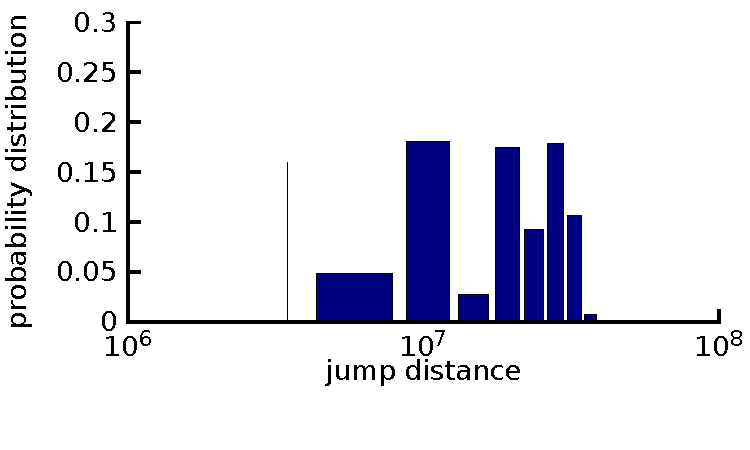
\includegraphics[scale=0.6]{tracechar-figures/3-day/webvm-jump-dist-distrib-readonly-appended-3-prob.pdf}}
% 	\hfill
% 	\subfloat[Jump distance distribution for block writes]{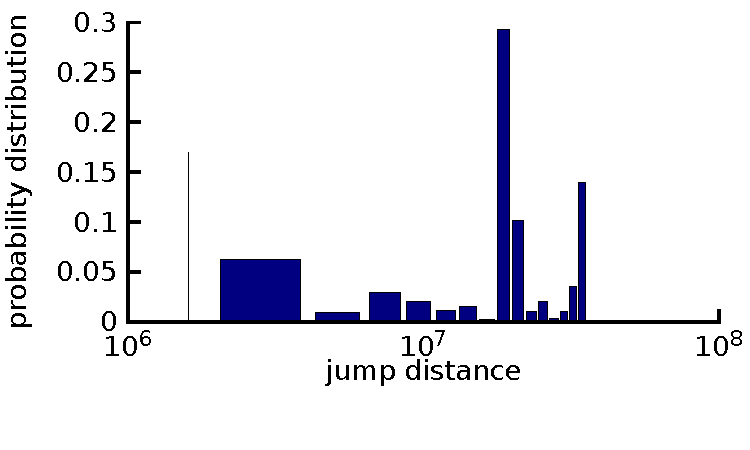
\includegraphics[scale=0.6]{tracechar-figures/3-day/webvm-jump-dist-distrib-writeonly-appended-3-prob.pdf}}
% 	\label{fig:webvm-jumpdist-read-write-distrib}
% \end{figure}

\begin{figure}
	\centering
	\subfloat[Jump distance distribution for \textit{webvm} trace]{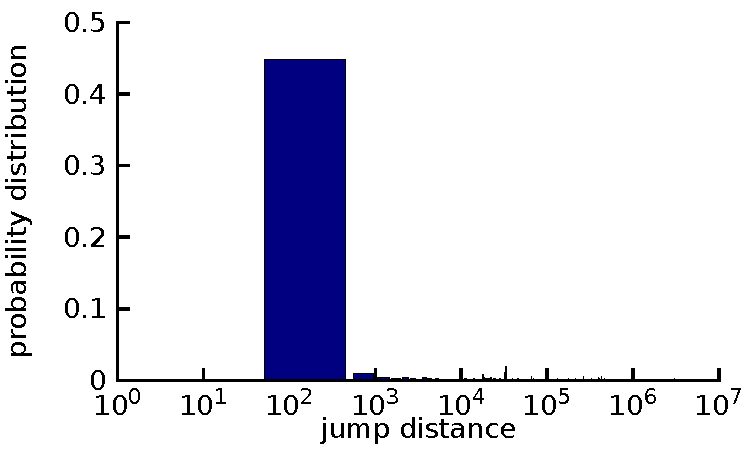
\includegraphics[scale=0.6]{tracechar-figures/21-day/webvm-jump-dist-distrib-readwrite-appended-21-prob.pdf}}
	\hfill
	\subfloat[Jump distance distribution for \textit{homes} trace]{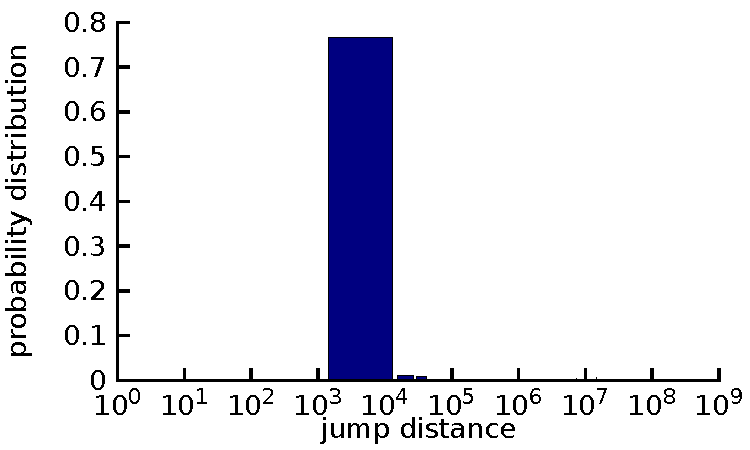
\includegraphics[scale=0.6]{tracechar-figures/21-day/homes-jump-dist-distrib-readwrite-appended-21-prob.pdf}}
	\caption{Jump distance probability distribution for read/write trace of \textit{webvm} and \textit{homes}}
	\label{fig:jumpdist-read-write-distrib}
\end{figure}

Although for all of the above metrics, we had presented separate distribution
for reads and writes, here we present a single distribution for all reads
and write requests combined. This is similar to the approach adopted 
in \cite{case-for-nas-benchmarks} and makes sense because jump distance
is a characteristic of the access trace which indicates how randomly or
not, the blocks are accessed (read or written) in the workload.

Fig.~\ref{fig:jumpdist-read-write-distrib} presents the probabilistic jump
distance distributions for both the \textit{webvm} and the \textit{homes} traces.
We can see that the majority of jump distances in the \textit{webvm} trace lie
between 100 to 1000 whereas they are between 1000 to 10,000 for the \textit{homes}.
Moreover, the largest jump distance in the \textit{homes} trace is an order of magnitude
larger than the largest jump distance in the \textit{webvm} trace. This is possibly
because the filesystem of the \textit{homes} system is similarly 
larger (470 GB) than the \textit{webvm} system (70 GB),
as mentioned earlier in Table~\ref{tab:tracechar-summary-stats}.

In this section, we described various characteristics of the I/O traces and 
quantified their content-defined versions for the available \textit{homes} and
\textit{webvm} traces. In the next section, we make the case that we need to
use such characterization to generate synthetic traces for evaluating new
I/O deduplication techniques comprehensively.


\section{The need for I/O deduplication benchmarks}
\label{sec:architectingchap-case}
% \begin{figure}[t]
% % 	\centering
% % 	\hspace{-0.7in}
% 	\subfloat[Markov model from \cite{storagecharacterization}]{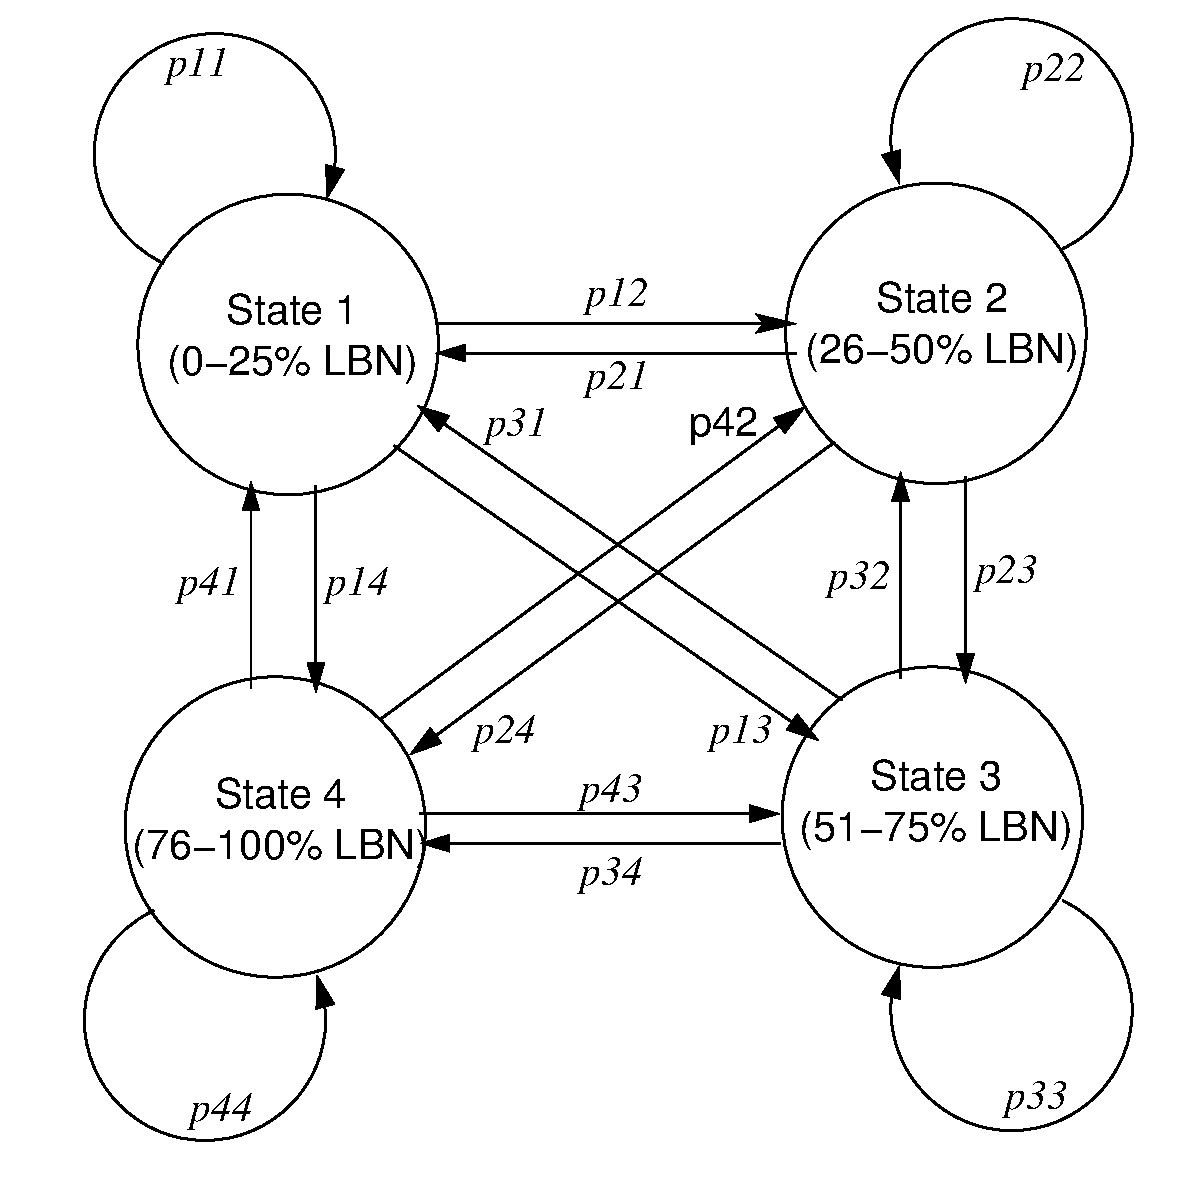
\includegraphics[scale=0.55]{presyn-figures/storagecharacterization.pdf}} \\
% 	\subfloat[Hierarchical Markov model from \cite{storagereplay,storagemodeling,decoupling-dc-studies}]{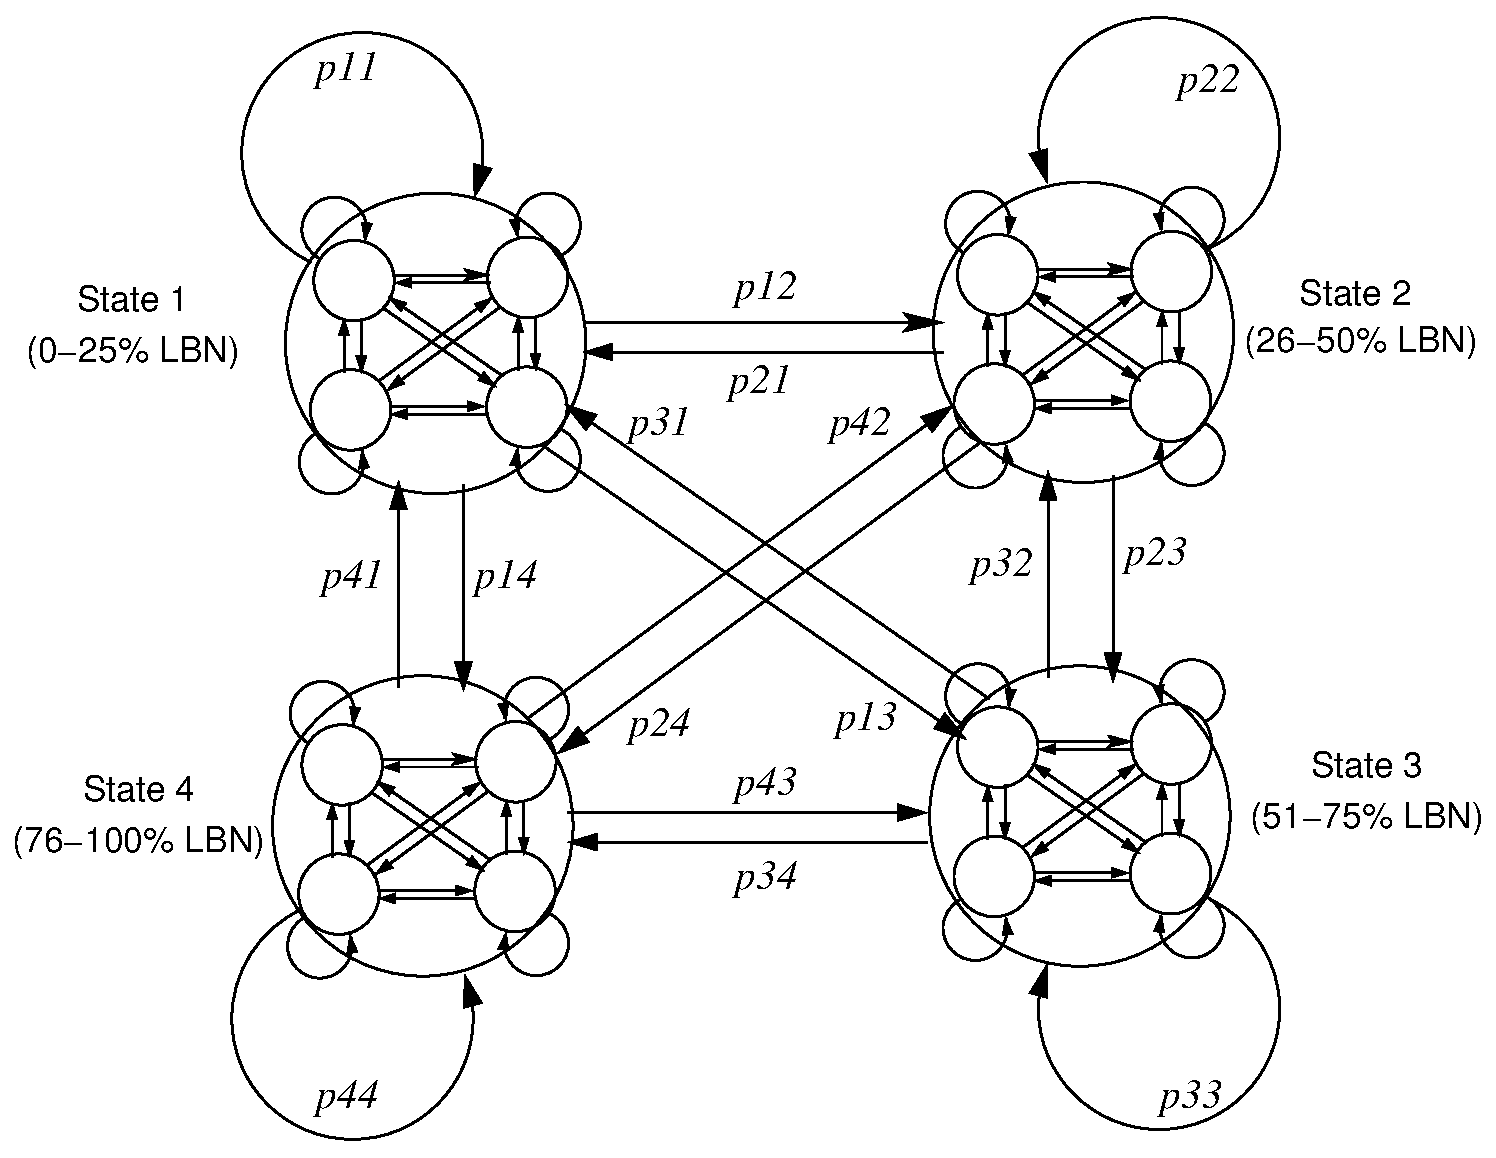
\includegraphics[scale=0.55]{presyn-figures/decoupling-dc-studies.pdf}}
% 	\caption{Using Markov models to capture the block accessed distribution~\cite{storagecharacterization, storagemodeling, storagereplay, decoupling-dc-studies}}
% 	\label{fig:storagecharacterization}
% \end{figure}

\begin{figure}[t]
	\centering
	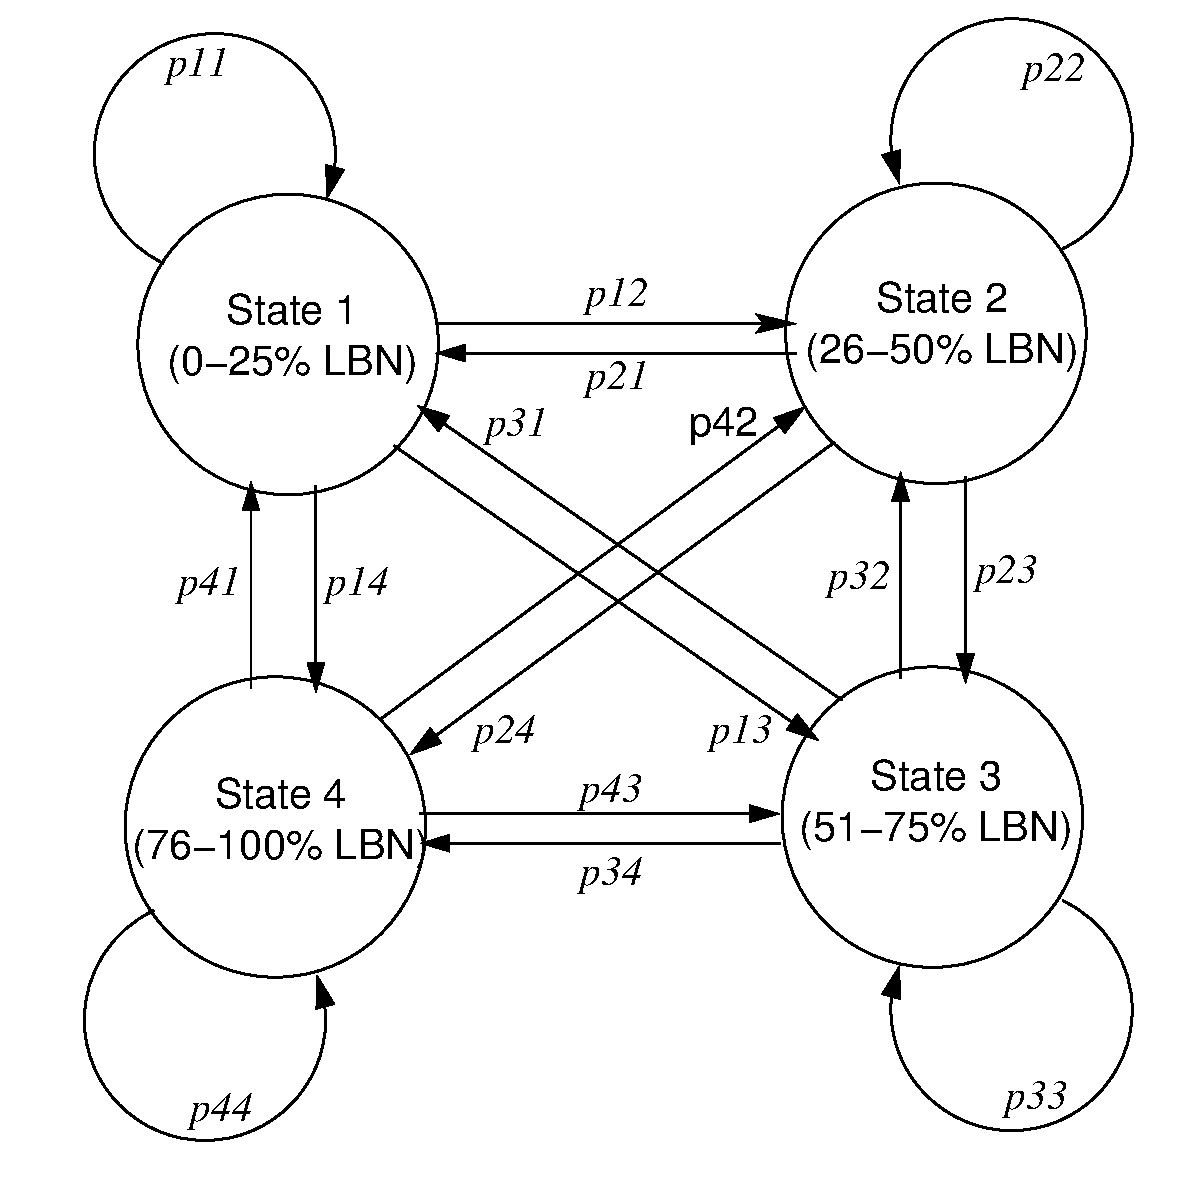
\includegraphics[scale=0.4]{presyn-figures/storagecharacterization.pdf}
	\caption{Markov model from \cite{storagecharacterization}: 
		Each arrow \textit{pij} represents probability of transition from one LBN 
			range (state \textit{i}) to itself or another (state \textit{j})}
	\label{fig:storagecharacterization}
\end{figure}


Recently, there has been significant research momentum in the direction
of surveying existing benchmarks and datasets to determine whether
enough realistic datasets or workloads are available for faithful
comparison and evaluation of competing storage optimization 
techniques~\cite{generating-datasets}.
In particular, the fields of I/O performance benchmarking as well as
storage deduplication characterization have been found wanting
with regards to availability of realistic benchmarks and datasets.
In this section, we make the case that there is significant
literature in the areas of realistic benchmark generation for 
network~\cite{echo} and 
storage I/O performance~\cite{storagecharacterization, storagemodeling,
storagereplay, flexi-replay, decoupling-dc-studies,
case-for-nas-benchmarks, jump-based-synthetic, distiller} as well as storage deduplication
evaluation~\cite{generating-datasets}, but none in the area of I/O deduplication. 

Basically, 
the I/O trace characterization and benchmark generation efforts 
focus on the request inter-arrival times as well as the spatial
and temporal locality of the access traces whereas the storage
deduplication benchmark generation effort focuses on modeling
the content duplication across temporal snapshots of the same
dataset. On the other hand, the requirement for I/O deduplication
benchmarks is a merging of the above two types of work, such 
that both the spatial/temporal locality aspects as well as
the duplicate content aspect be characterized and captured 
in the benchmark realistically. In the rest of this section,
we describe the existing work in realistic benchmark generation
under each of the categories of (i)~Storage I/O, 
(ii)~Network I/O activity, 
(iii)~File system metadata,
and
(iv)~Storage data deduplication.




\subsection{Generating realistic storage I/O performance benchmarks}
The generation of realistic I/O performance benchmarks
has received considerable attention in recent literature~\cite{storagecharacterization, storagemodeling,
storagereplay, flexi-replay, decoupling-dc-studies,
jump-based-synthetic, distiller}. 
The work in~\cite{storagecharacterization}
builds a Markov model to capture \textit{spatial locality},
with each state representing one-quarter of the 
block address range (called logical block number range or LBN range) 
and each transition representing
the probability of transitioning from one LBN range to another. The idea
is that due to the spatial nature of the workload, most of the
transitions would stay within the same state and the probabilities
of transitioning out of one state to another would be quite low. 
Thus, a request stream is perceived as a state machine 
which transitions between LBN ranges with certain probabilities.


Fig.~\ref{fig:storagecharacterization} is a reproduction of
the Markov model built in \cite{storagecharacterization}, and as
can be seen, the model has 4 states and 16 transitions between
the states. The probability of each transition in this model
is determined by characterizing real-world traces, and could
be workload-specific (i.e., dependent on the type of workload
that needs to be captured by the model). The traces used were
for web services like a message store for an email service, 
image tile storage for a large-scale geo-mapping service, and 
a blob storage service which hosted huge amounts of user-generated
content~\cite{storagecharacterization}.

\begin{figure}[t]
	\centering
	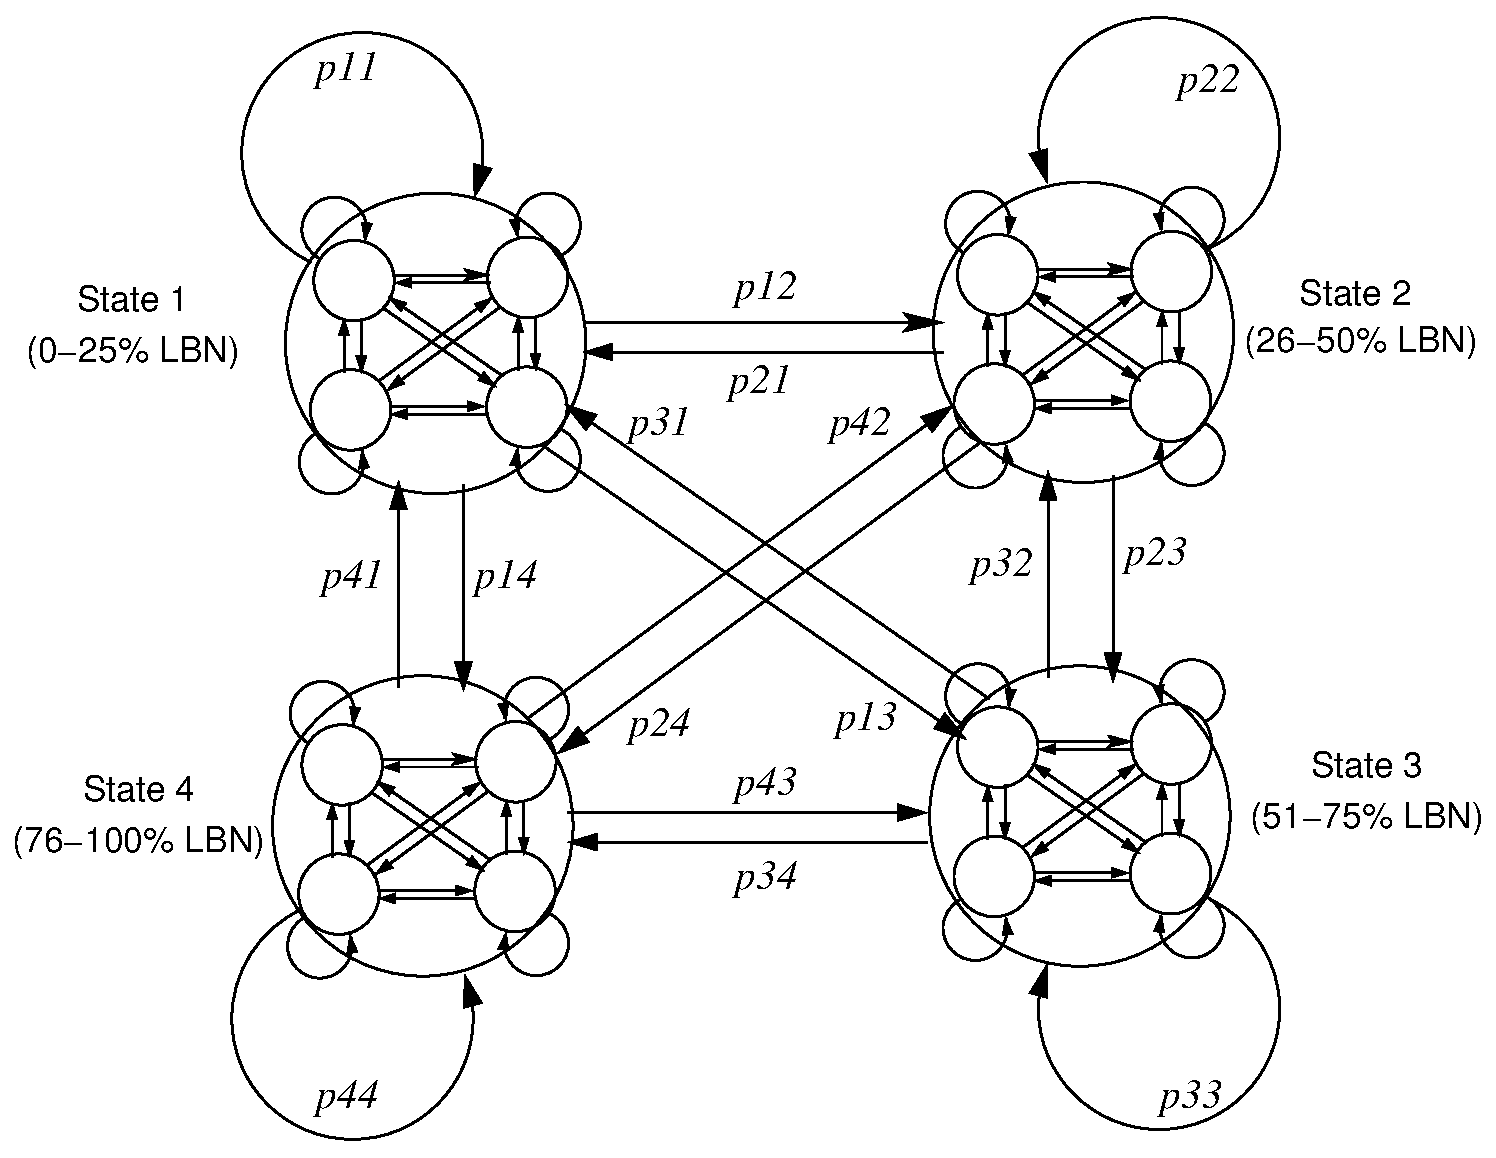
\includegraphics[scale=0.5]{presyn-figures/decoupling-dc-studies.pdf}
	\caption{Markov model from \cite{decoupling-dc-studies}: Each arrow \textit{pij} represents 
		probability of transition from one LBN
	range (state \textit{i}) to itself or another (state \textit{j}). Also, each state \textit{i}
	is further divided into 4 sub-states each, having internal transition probabilities as well.}
	\label{fig:decoupling-dc-studies}
\end{figure}


The work in~\cite{storagereplay, storagemodeling, decoupling-dc-studies}
builds on top of the above Markov model idea by building a hierarchical
Markov model such that each of the above states is further divided 
into 4 finer granularity states. For example, the LBN range
0-25\% from Fig.~\ref{fig:storagecharacterization} is broken
into 4 sub-ranges like 0-6.25\%, 6.25-12.5\%, 12.5-18.75\% 
and 18.75-25\%. Pictorially, the hierarchical Markov looks as
depicted in Fig.~\ref{fig:decoupling-dc-studies}, although
the inner states have not been marked with all the LBN sub-ranges therein.

Representing the storage I/O model as a hierarchical Markov model
enables to represent information of a finer granularity than \cite{storagecharacterization}.
Thus, the two level diagram has a total of 16 states and 76 transitions,
which are once again parameterized using a thorough characterization
of available real-world storage I/O traces.

The work in \cite{jump-based-synthetic} claims that to characterize
and recreate a realistic storage I/O workload, it is necessary to not
only capture the block accessed distribution, but also the jump distance
distribution. In view of this, the approach proposed in \cite{jump-based-synthetic}
is to transform the synthetic trace generation problem into the
Hamiltonian Path problem, and then to apply a brute-force, depth-first
search to find a Hamiltonian path (this path is expected to have the
same jump distance characteristics as the original trace). 
However, if a complete Hamiltonian
Path is not found, approximation techniques are used to construct 
the access pattern. The evaluation therein shows that if the
trace to be generated needs to have less than 150 I/O requests, only
then this brute-force approach is able to find complete Hamiltonian
paths\textemdash{}in most other cases, the algorithm is forced to rely on
the latter approximation techniques. 

The work in \cite{distiller} hypothesizes that although synthetic workloads
are flexible and easy to obtain, the challenge is that synthetic
workloads are accurate only if they share certain key properties
with the original production workload(s). The unfortunate aspect
here is that we do not know which properties are ``key'' for
any given workload or storage system. Thus, regarding the selection
of key properties for workload characterization
and generation, the work in \cite{distiller} presents a tool
called \texttt{Distiller} that can automatically identify
them using an iterative trial-and-error method. As input, the
\texttt{Distiller} tool needs a library of workload attributes, 
from which it picks one additional attribute at each iteration,
and checks whether the chosen set of attributes is representative
enough of the given workload. If so, the modeling is done and
if not, it chooses one more attribute in the next iteration
and so on until a realistic representation is achieved.

\subsection{Realistic network activity modeling and benchmark generation}
The work in \cite{echo} presents a modeling scheme called ECHO, which 
captures the temporal and spatial behaviour of network traffic in
large-scale datacenter applications. Two models are built, wherein
the first is a distribution-fitting model (called the \textit{single-server temporal
model}) that generates per-server
network traffic and the second is a Markov chain model (called the \textit{system-wide
spatial model}) that captures
server-to-server interactions. 

The single-server temporal model of \cite{echo} consists of using
a network trace as an input and identifying known distributions\textemdash{}Gaussian,
Poisson, Zipf, etc\textemdash{}in the network activity pattern. The output 
mathematical expression from this model would be a superposition of
multiple known distributions such that sampling of this composite
distribution allows to generate network activity patterns that have
similar temporal patterns as the ones present in the original trace.
However, this method captures the network activity only for
individual servers and can not address server-to-server activity
patterns or network traffic across sets of machines.

\begin{figure}[t]
	\centering
	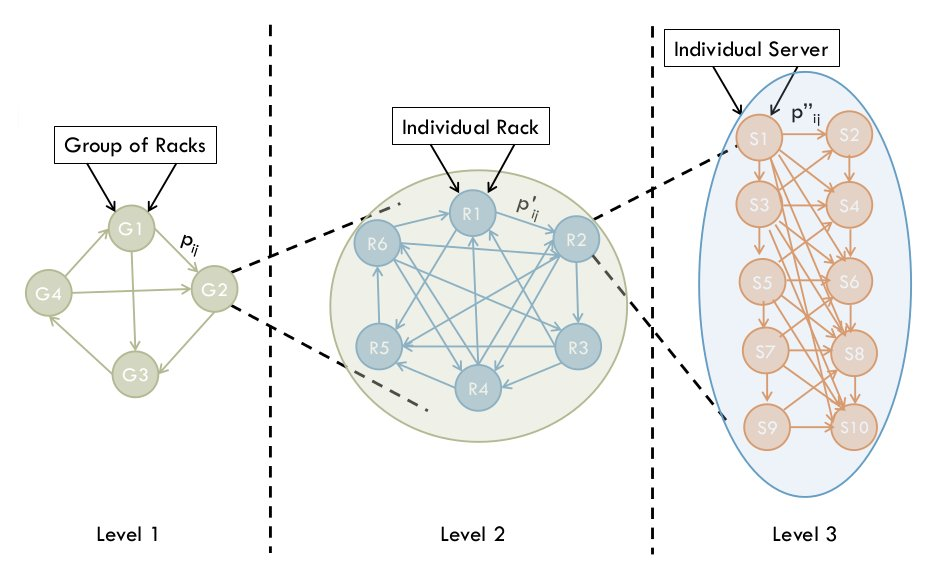
\includegraphics[scale=0.4]{presyn-figures/echo.jpg}
	\caption{Schematic of the hierarchical spatial Markov chain model~\cite{echo}}
	\label{fig:echo}
\end{figure}

The second model developed in \cite{echo} is a hierarchical Markov
chain model which captures the network activity patterns for
individual servers, across servers within a rack, as well as
across racks within a group of racks. Fig.~\ref{fig:echo} is 
a lifted reproduction from \cite{echo} of the schematic of
the hierarchical spatial Markov chain model. 
As can be seen, this model is hierarchical, and 
the level of detail in the model can be adjusted according to the
requirements of each application.

\subsection{Generating realistic file system benchmarks}
Similar to the quest in \cite{distiller} regarding the key properties 
of a given workload, the work in \cite{impressions} is motivated by
the key properties needed to realistically represent a file system
image. The claim therein, is that, depending on the workload to
be emulated or evaluated, the file system image to be used may
need different levels of detail. For example, a data mirroring
scheme like RAID or a system that takes full backups would be
independent of both metadata and content of the filesystem.
On the other extreme, a desktop search engine's performance
would depend on both the metadata and the exact content of
the file system on which it operates.

Although the work in \cite{impressions} does not address the evaluation
or analysis of deduplication techniques, the framework (called \textit{Impressions})
presented therein would be useful to capture the content profile
of any real file system such that deduplication techniques can
be evaluated over it~\cite{generating-datasets}.

\subsection{Generating realistic storage deduplication benchmarks} 
To justify the creation of benchmarks for storage deduplication, the work in
\cite{generating-datasets} claims that the benchmark or datasets should be
such that they should be :-
\begin{enumerate}
		\singlespacing
	\item Sufficiently large
	\item Having controllable characteristics
	\item Easy to distribute to other researchers
	\item Easily accessible or reproducible by other researchers
	\item Realistic
\end{enumerate}

The requirement of ``realistic'' datasets is straight-forward\textemdash{}unless the
dataset is realistic, there is no way to judge whether any proposed 
technique is useful in the real world. 
However, if the dataset is ``realistic'' because it contains proprietary
or private information, then the owner of the dataset may be reluctant to
make the dataset publicly available. Further, the requirement
that the dataset is sufficiently large, is also at crossroads with the 
requirement that the dataset be easily accessible to other researchers,
because larger the dataset, tougher the task of hosting and maintaining
it online.

Due to above conflicting requirements, the work in \cite{generating-datasets}
suggests a framework which involves capturing the important characteristics
of a real-world workload into a model which can be represented with a much
smaller storage footprint than the actual workload, and hence can be easily
distributed across research groups. The work in \cite{generating-datasets}
generates benchmarks which capture the changes in file system across multiple
snapshots (referred to as \textit{mutation}) along-with its content 
representation, using a combination of a 
Markov model and a multi-dimensional distribution model.

The work in \cite{dedis} presents DEDISbench, a realistic storage
deduplication benchmark. 
The I/O generation framework in DEDISbench consists of two
components: (i) Access pattern generator, and (ii) Content generator.
The access pattern generator can generate sequential, uniform-random
or random-with-hotspots accesses depending on user choice.
The random-with-hotspots access pattern
uses TPC-C NURand function to simulate
access hotspots in write requests\textemdash{}access hotspot implies that
a few blocks will be accessed multiple times while other blocks may 
only be accessed once each. 
If the request is a write request, the
content generator generates the random content to be written to 
the specified block, based on an input distribution of 
duplicates.
A tool called DEDISgen is also
presented~\cite{dedis}, which can be used to compute the cumulative
distributions of block accesses for a real filesystem such that 
this distribution can be used as an input to DEDISbench for generating
the realistic benchmarks for storage deduplication.

Since our requirement is to evaluate read I/O deduplication techniques,
and not storage deduplication, hence to use DEDISbench, we would need
to tweak it such that access hotspots are created for read accesses
as well, and not just for write requests. 
Moreover, the realistic nature of not only the content in the 
filesystem (i.e., on storage) but also the content in the 
read I/O (i.e., in I/O traces)
needs to be captured. Specifically, DEDISbench uses the duplicate
distribution to guide the content generation for write requests.
We need the read access hotspots to also be similarly guided by
a duplicate distribution of content present in real I/O 
traces\textemdash{}basically
to capture the dual metrics of \textit{sharing factor} and 
\textit{occurrence factor} of every content in the trace.
\\
\\
Based on the above surveyed literature, we conclude that there are no
realistic benchmarking tools or trace generation frameworks that can
be used for evaluation of I/O deduplication techniques. Thus, for the 
evaluation of such techniques, researchers need to either collect multiple
production workload traces for their own research, or create frameworks
that can synthesize realistic I/O traces along-with content representation.
% In the next sub-section, we present some potential ideas for building
% controllable synthetic traces for I/O deduplication analysis, with 
% the caveat that actually building such traces and using them for 
% evaluation would again require access to certain realistic workloads,
% and hence is beyond the scope of this thesis.
% 
% \subsection{Proposed approach for generating controllable, realistic I/O workloads with duplicate content}
% details pending


\section{Conclusions}
The purpose of this literature review was to find publicly-available 
datasets of I/O traces with content representation, that could be 
used in evaluation of our DRIVE dedup system. However, our survey 
revealed that among the publicly-available datasets, only the ones 
available via IODEDUP paper~\cite{iodedup} have content representation, 
and we have already used them for our evaluation in the previous chapter. 

The obstacle that we faced in doing a real implementation study for the 
DRIVE system is that neither were we able to procure production I/O 
workloads or traces, nor could we find any tools that would generate 
realistic traces with duplicate I/O content. In fact, this obstacle 
is the basis for this chapter, which is basically a detailed survey 
of the available traces, workloads and tools related to disk and I/O 
deduplication. We wish to restate that this chapter is not intended 
as a design contribution. Its intent is to make the case that a 
comprehensive tool is needed that can generate realistic 
workloads/traces which have significant levels of I/O deduplication, so 
that it can be used for evaluating various I/O deduplication approaches.
